\chapter{Results and discussion}\label{sec:results}

The fundamental goal of this project is to assess the suitability of posterior
agreement as a robust model selection criterion in the image classification setting.
This section will outline the principal results in a deductive way, starting with an 
empirical exploration of the robustness properties of the PA kernel and culminating
with performance results in benchmark datasets.

\section{PA as a robustness metric}\label{sec:results_robustness}

\subsection{Empirical behaviour}

Starting from the simplest possible setting, we will explore the behavior of the metric 
under different levels of sample mismatch. More specifically, we will assess the performance 
of perfect, random, and constant binary classifiers by manipulating a 
Bernoulli sample and simulating different levels of prediction confidence.

\begin{figure}[H]
    \centering
    \begin{subfigure}[b]{0.45\textwidth}
        \centering
        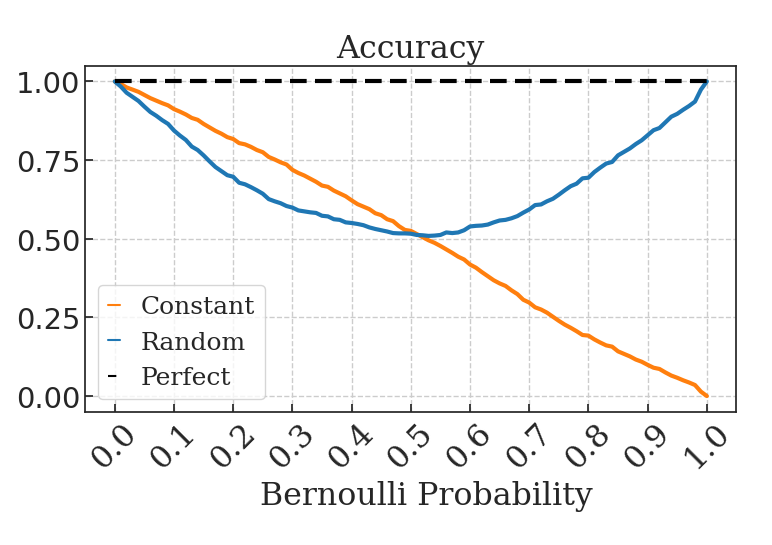
\includegraphics[width=\textwidth]{img/results_discussion/empirical/artificial_acc_final.png}
    \end{subfigure}
    \hfill
    \begin{subfigure}[b]{0.45\textwidth}
        \centering
        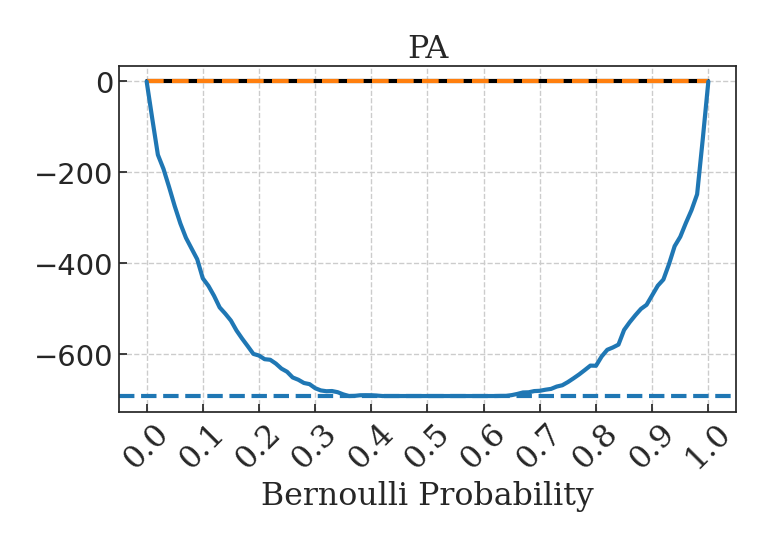
\includegraphics[width=\textwidth]{img/results_discussion/empirical/artificial_logPA_final.png}
    \end{subfigure}
    \caption{Evolution of performance and robustness for the three classifiers}
    \label{fig:empirical_plot}
\end{figure}

A $N=1000$ Bernoulli sample was generated with a symmetrical confidence level 
of prediction $\pm \Delta/2$. For $p=0.5$, the metric achieves its minimum 
value $N \log{1/2}$ for the random classifier, as $\beta = 0$, and tends to its maximum
value of $0$ as $\beta \longrightarrow \infty$.

\begin{table}[H]
    \centering
    \begin{tabular}{lccc}
    Classifier & Accuracy & $\beta$ & PA \\
    \midrule
    Perfect   & 1.000     & 12.331  & $-0.0088218$ \\
    Constant  & 0.525     & 12.331  & $-0.0088218$ \\
    Random    & 0.516     & 0.000   & $-693.14$    \\
    \bottomrule
    \end{tabular}
    \caption{Comparison of classifier performance metrics for $p = 0.5$.}
    \label{tab:empirical_table}
\end{table}

The random classifier sample was generated by permuting the original so 
that the number of mismatched observations depends on the bernoulli probability $p$. 
As we can see, the theoretical miniumum value  is obtained only after
a certain perturbation threshold has been reached. This illustrates the trade-off
navigated during the kernel optimization, in which matching samples penalize the 
metric value the lower the value of $\beta$ is, whereas mismatching samples will
penalize the overall value the further from zero $\beta$ is. Given the highly non-linear
nature of the logarithm in the interval $[0,1]$, the metric will penalize 
disagreement much more than agreement, as shown in Figure \ref{fig:empirical_plot}.
A truly random classifier (i.e. balanced on the two classes) would yield the minimum
PA value for any possible original sample, as shown in the blue dashed line.\\

One of the most relevant differences between posterior agreement and any accuracy-based
measure, as discussed in previous chapters, is the fact that its assessment is based on
the whole probabilistic output of the model, and therefore can be used as a measure of
confidence in the predictions. The prediction confidence, expressed as a difference in 
the unnormalized log-odds (commonly known as logits), is very informative with regard 
to the quality of the model, as we can intuitively infer that the latent 
space represented by a high-confidence model encodes a better set of features 
to discriminate observation classes than one with a lower prediction confidence. \\

For instance, when comparing two models of similar predictive power but at different 
confidence levels, maximum posterior agreement will be achieved with a higher 
$\beta^{*}$ for the model that tends to yield more flattened distributions. This
information is especially valuable in the covariate shift setting, given that robust
models that rely on less accessible sets of features will most likely yield conservative
predictions on in-distribution samples, but at the same time keep a high prediction
power on out-of-distribution observations. \\

\begin{figure}[H]
    \centering
    \begin{subfigure}[b]{0.45\textwidth}
        \centering
        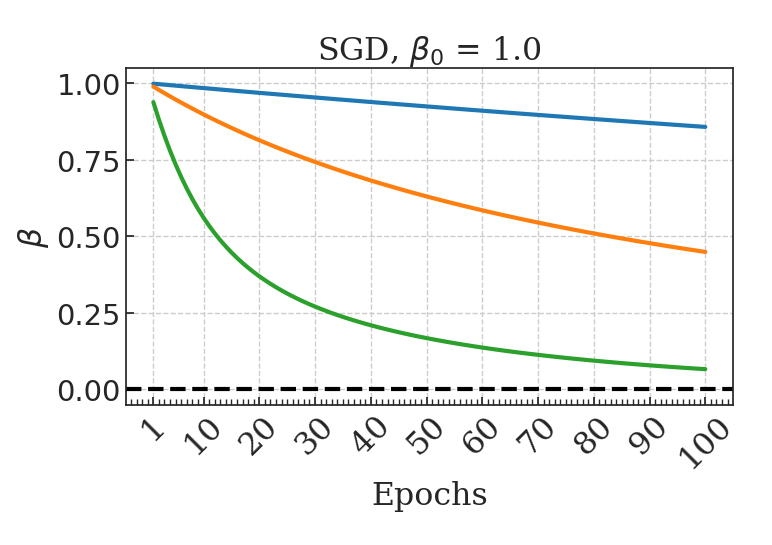
\includegraphics[width=\textwidth]{img/results_discussion/empirical/nonrob_met=betas_hue=ldiff.png}
    \end{subfigure}
    \hfill
    \begin{subfigure}[b]{0.45\textwidth}
        \centering
        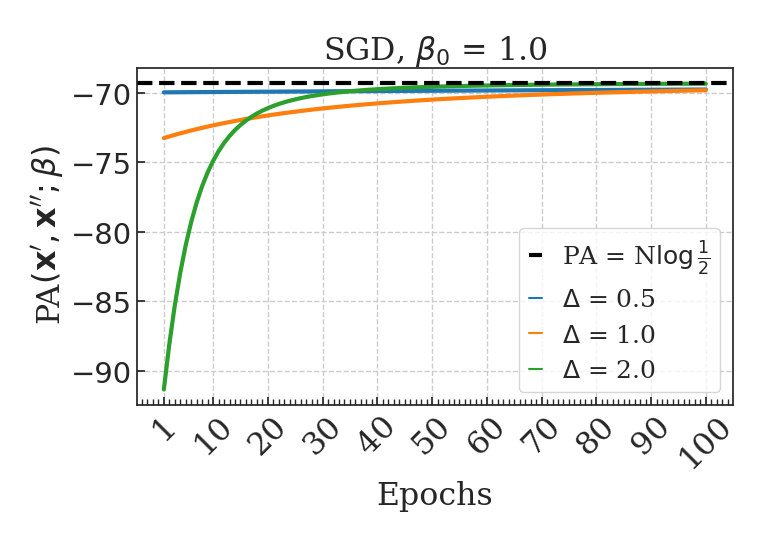
\includegraphics[width=\textwidth]{img/results_discussion/empirical/nonrob_met=logPA_hue=ldiff.png}
    \end{subfigure}
    \caption{Evolution of PA kernel optimization under different levels of prediction 
    confidence. An illustration of the original log-odds and its associated posterior distribution
    can be found in Appendix \ref{subsec:appendix_empirical_behaviour}.}
    \label{fig:prediction_confidence}
\end{figure}

These and other results (see Appendix \ref{subsec:appendix_empirical_behaviour}) indicate
that the PA kernel behaves as expected and is highly informative of the generalization
capabilities of the model, provided that the nature of the randomness existing
between $\bm{x}^\prime$ and $\bm{x}^{\prime \prime}$ is known.

\subsection{Robustness assessment to sampling randomness}

The results obtained with artificial samples motivate the exploration of more realistic
scenarios. In general, the PA metric is expected to capture the generalization capabilities
of any model yielding probabilistic predictions, regardless of the task at hand. This
already represents an incredible advantage from an epistemological perspective, as we
can argue that the metric is agnostic of the underlying mechanism that generated the data
and even to the nature of the data itself. \\

In order to verify this claim, we will start by evaluating the robustness of two
different classifier models in two different domains under increasing levels of 
white noise perturbation. This particular setting, even if highly artificial, is 
relevant in any classification context, as it represents general measure of the 
quality of the features learned by the model. The presence of white noise, at least 
at low levels, does not perturb the set of features that define a particular class from
a human perspective, and should therefore not perturb very significantly the
predictions yielded by the model. \\

HERE THE PLOT OF THE LEVENSHTEIN DISTANCE PLOT HERE. \\

A sentiment classifier analysis. In this case, the random nature of the noise perturbations
is shown to exploit specific vulnerabilities of language models, which paradoxically 
have been shown to be robust to more highly crafted perturbations, such as changes in
language or replacement of complete words. \\

\begin{figure}[H]
    \centering
    \begin{subfigure}[b]{0.45\textwidth}
        \centering
        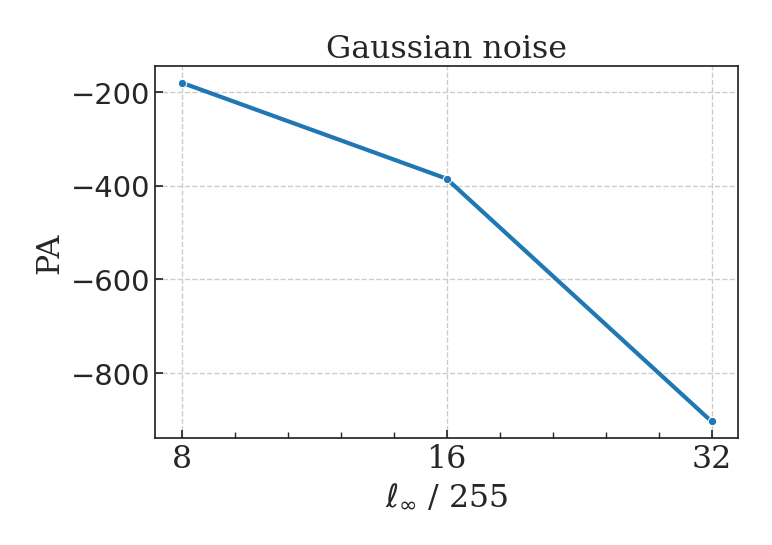
\includegraphics[width=\textwidth]{img/results_discussion/adversarial/GAUSSIAN_logPA_eps_single.png}
    \end{subfigure}
    \hfill
    \begin{subfigure}[b]{0.45\textwidth}
        \centering
        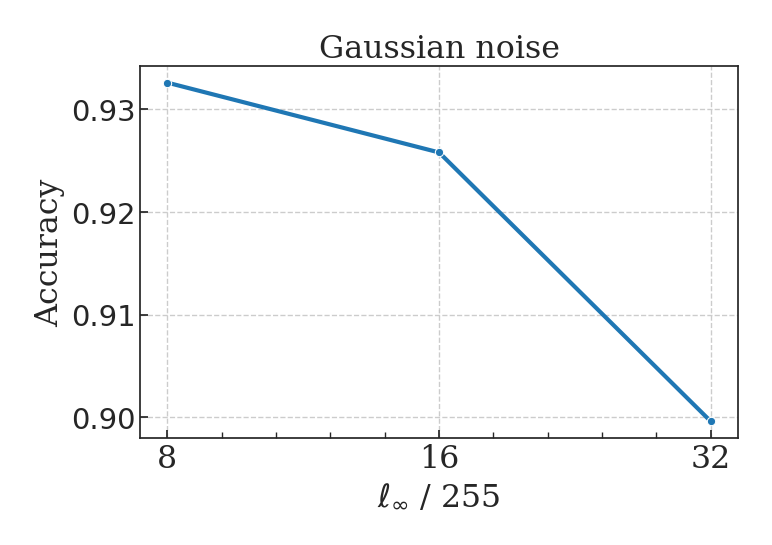
\includegraphics[width=\textwidth]{img/results_discussion/adversarial/GAUSSIAN_acc_pa_eps_single.png}
    \end{subfigure}
    \caption{PA and accuracy of CIFAR10 classification for increasing levels of white noise intensity.}
    \label{fig:gaussian_noise}
\end{figure}

In this second example, a 10.000 observation sample of CIFAR10 images was perturbed
with white noise at different levels of intensity. The magnitude of the perturbation
is expressed in the same terms as those of an adversarial 
attack (see Section \ref{sec:adversarial_setting}) for further 
reference, but translate to using $\sigma = 3 \ell_\infty$, as 99.73\% of the
total mass of the gaussian distribution lies within the interval $\pm 3\sigma$. \\

As expected, PA is highly sensitive to the presence of white noise,
and is able to capture the generalization capabilities of the model in a much more
informative way than accuracy. We can obtain a higher understanding of the degree of
sensitivity of the metric if we adjust the perturbation so that if only affects
a certain ratio of observations. \\

\begin{figure}[H]
    \centering
    \begin{subfigure}[b]{0.49\textwidth}
        \centering
        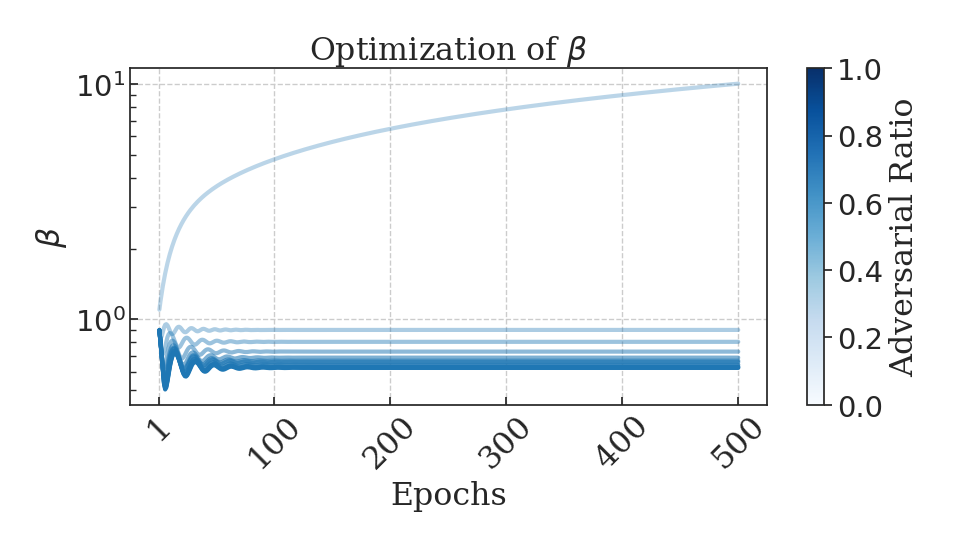
\includegraphics[width=\textwidth]{img/results_discussion/empirical/betas.png}
    \end{subfigure}
    \hfill
    \begin{subfigure}[b]{0.49\textwidth}
        \centering
        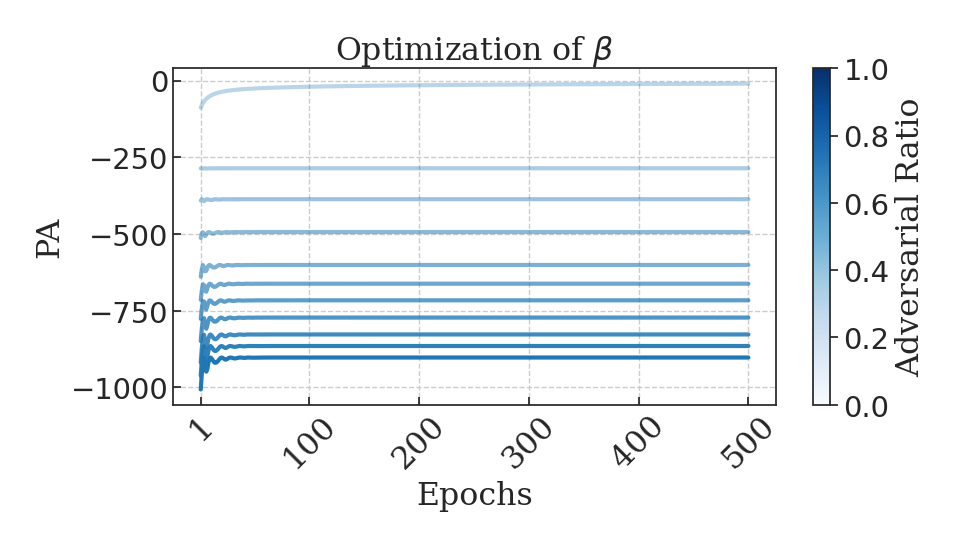
\includegraphics[width=\textwidth]{img/results_discussion/empirical/logpas.png}
    \end{subfigure}
    \caption{PA kernel optimization in the CIFAR10 gaussian noise setting for different ratio
    of perturbed samples. Perturbation magnitude is $\ell_\infty$ = 32 / 255.}
    \label{fig:gaussian_optimization}
\end{figure}

As expected, $\beta$ tends to infinity in the unperturbed case, and converges
quickly to its optimal value in the rest of cases, even if the sample size is considerably
large and memory-intensive. The decay in the PA value is less pronounced the higher
fraction of perturbed samples are there, as we observed in the artificial setting, which
is consistent with the concept of robustness itself, as it already approaches
the lower bound for these kinds of perturbation even when the whole sample has yet not
been perturbed. \\

\section{Adversarial setting}\label{sec:results_adversarial}

The first scenario in which covariate shift robustness will be tested is the
adversarial setting. This setting serves as an archetypal 
use case for any robustness metric, given that adversarial perturbations are
deliberately generated to mislead the model. By definition, the higher the
effectiveness of the attack, the lower the robustness score of the model. In particular, 
PA should be highly informative about the defensive capabilities of the model, as the posterior 
distribution over the hypothesis class will shift significantly in the 
presence of adversarial perturbations. This section aims to validate 
this claim and provide deeper insights into the nature of the metric. \\

It is important to note that adversarial perturbations constitute an
intermediate setting between sampling randomness and distribution shift. 
On the one hand, they emulate a sampling variation that appears 
as an outlier under the model's representation of the true class, even if
the source of variability is completely artificial. On the other
hand, samples are known to contain the set of features that should 
align with the inductive bias of the model, and so the model's ability to 
distillate those features is in question. In practice, we are evaluating the 
quality of the complex discriminator function defining a basin of stability
around original samples, and for that no deep understanding of the nature of 
the randomness of the samples or the features they encode is needed.\\

This interpretation is aligned with the measure provided by accuracy-based metrics, 
because adversarial samples are not expected to contain any relevant features of other
classes or express any accountable source of randomness, but instead exploit specific
vulnerabilities of models to specifically alter the position of the maximum of 
the posterior ditribution. A greater posterior overlap will still
indicate higher robustness to attacks, regardless of the nature of the model or the
attack, but optimal posteriors are expected to converge to very peaked gibbs
distributions centered at the predicted class, reducing the interpretability of PA
to that of accuracy. \\

In order to explore these claims, robustness and performance results will be
provided through the adversarial fidelity ratio (AFR) value and compared to those
yielded by PA. The AFR computed with the true class labels will be used as a baseline
of model performance, whereas the AFR computed with the predicted class label
will be a reference for robustness, as it aligns with the aforementioned
interpretation.

\begin{definition}[Adversarial fidelity ratio]
    Let $\bm{\hat{y}^\prime}, \bm{\hat{y}^{\prime\prime}} \in \mathcal{Y}^N$ be the predicted class 
    labels for $\bm{x}^\prime$ and $\bm{x}^{\prime \prime}$, respectively, 
    and $\bm{y}\in \mathcal{Y}^N$ the true labels. Let $\operatorname{ACC}$ be the standard accuracy 
    metric, as defined in Section \ref{sec:robustness_to_covariate_shift}.
    The adversarial fidelity ratio (AFR) is expressed as

    $$
    \begin{aligned}
        \operatorname{AFR (T)} &= \operatorname{ACC}(\bm{\hat{y}^{\prime \prime}}, \bm{y}), \\
        \operatorname{AFR (P)} &= \operatorname{ACC}(\bm{\hat{y}^{\prime \prime}}, \bm{\hat{y}^{\prime}}).
    \end{aligned}
    $$

\end{definition}

The results provided in this section have been obtained using the CIFAR10 dataset CITE1,
which is widely regarded as a standard benchmark for robustness evaluation. CIFAR10 is
a balanced dataset containing 60.000 coloured 32 $\times$ 32 pixel images belonging to 10
different classes. We will consider a pre-trained WideResNet-28-10 as a baseline, undefended
model and compare it to some state-of-the-art robust models provided by the 
RobustBench CITE2
library under PGD CITE3
and FMN CITE4
attacks, both run for a thousand steps (see Section \ref{sec:adversarial_setting}). 
The PGD attack power will be specified in terms of $\ell_\infty$, which corresponds
to the maximum perturbation allowed for each pixel. This is consistent with the characterization
of adversarial perturbation given in the previous chapter, as every perturbation will be bounded
to the region defined by $\mathbf{B}_\infty^{\ell_{\infty}} (x)$.

\begin{figure}[H]
    \centering
    \begin{subfigure}[b]{0.25\textwidth}
        \centering
        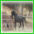
\includegraphics[width=\textwidth]{img/results_discussion/adversarial/adv_unperturbed_framed.png}
        \caption{Original}
    \end{subfigure}
    \hfill
    \begin{subfigure}[b]{0.25\textwidth}
        \centering
        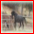
\includegraphics[width=\textwidth]{img/results_discussion/adversarial/adv_pgd_framed.png}
        \caption{PGD, $\ell_\infty$ = 36/255}
    \end{subfigure}
    \hfill
    \begin{subfigure}[b]{0.25\textwidth}
        \centering
        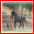
\includegraphics[width=\textwidth]{img/results_discussion/adversarial/adv_fmn_framed.png}
        \caption{FMN}
    \end{subfigure}
    \caption{Original and adversarially perturbed CIFAR10 sample. Both perturbations succeed
    at misleading an undefended pre-trained WideResNet-28-10 net.}
\end{figure}

Besides the maximum norm allowed for each perturbation, we are also interested in evaluating 
the sensitivity of our robustness measure to the ratio of perturbed samples in the dataset, 
also known as adversarial ratio (AR). The final adversarial dataset $\bm{x}''$ will be generated as

$$
\bm{x}'' := \operatorname{AR} \bm{x}'' + (1 - \operatorname{AR}) \bm{x}',
$$

where $\bm{x}'' = \bm{x}' + \bm{\Delta}$, as per Definition \ref{def:adversarial_perturbation}.
This incremental expansion of the attack is particularly relevant for PA, as we would initially 
expect it to behave non-linearly with respect to $\operatorname{AR}$ and converge faster to
the the $\operatorname{AR}=1$ robustness value than any accuracy-based metric, in light of the results obtained
in the previous section. We can quantify the model discriminability over increasing $\operatorname{AR}$
by computing the adversarial ratio gap $\Delta \operatorname{AR}$.\\

\begin{definition}[Adversarial ratio gap]
    Let $\gamma_+$ and $\gamma_-$ be two models, not necessarily different. Let $\operatorname{AR}_{+}$ and 
    $\operatorname{AR}_{-}$ be the adversarial ratio values such that

    $$
    \operatorname{PA}^{\gamma_+} \bigg|_{\operatorname{AR}_{+}} = \operatorname{PA}^{\gamma_-}\bigg|_{\operatorname{AR}_{-}}
    $$

    the aversarial ratio gap ($\Delta \operatorname{AR}$) is obtained as

    $$
    \Delta\operatorname{AR} = \operatorname{AR}_{+} - \operatorname{AR}_{-}. 
    $$
\end{definition}

Before delving into the results, it is worth exploring the immediate consequences
of the previous claim, namely the fact that the maximum posterior agreement will
be achieved when gibbs distributions are highly peaked on the predicted 
class, at least for moderately aggressive attacks. This is because most adversarial 
samples will not succeed at misleading the model and thus drive the inverse temperature to
infinity. The divergence of $\beta$ is only limited by the set of misleading adversarial 
samples, that for being perturbed from the original class are still expected to assign a
significant confidence to the original prediction, even if not the maximum anymore.
Table \ref{tab:entropy_gibbs} illustrates this claim by showing that $\beta^{*} > 1$ 
for all robust models, resulting in a substantial decrease of the entropy between initial and 
optimal posteriors. \\

\begin{table}[H]
    \centering
        \begin{tabular}{l|rr|rr}
        Defense & $\beta^{*}_{\text{PGD}}$ & $\Delta H_{\text{PGD}}$  & $\beta^{*}_{\text{FMN}}$ & $\Delta H_{\text{FMN}}$ \\
        \midrule
        {\color{tab:orange} \textbf{Undefended}} & 0.78 & 0.048 & 0.65 & 0.10\\
        {\color{tab:blue} \textbf{Engstrom et al.}} & 15.63 & -1.204 & 2.59 & -0.71\\
        {\color{tab:green} \textbf{Athalye et al.}} & 35.48 & -3.049 & 19.84 & -2.13 \\
        {\color{tab:red} \textbf{Wong et al.}} & 15.46 & -1.229 & 4.59 & -0.96\\
        {\color{tab:purple} \textbf{Addepalli et al.}} & 15.89 & -2.023 & 6.08 & -1.71 \\
        {\color{tab:brown} \textbf{Wang et al.}} & 11.24 & -1.833 & 2.53 & -1.41\\
        \bottomrule
        \end{tabular}
        \caption{
        Entropy difference $\Delta H = H(\beta^{*}) - H(\beta)$ in bits 
        for different models, obtained for FMN and $\ell_\infty$=8/255 
        PGD attacks, both at $\operatorname{AR} = 1$. Entropy values are 
        estimated using the average posterior distribution over correctly classified
        samples, which constitute the largest proportion of the dataset.
        Figures \ref{fig:pgd_distributions_undefended}-\ref{fig:pgd_distributions_bpda}
        show the initial and optimal average posteriors from which these values
        were computed.
        }
        \label{tab:entropy_gibbs}
\end{table}

This realization allows us to break down the dataset into subsets of observations
that contribute to the final PA value in different ways, and therefore improve
the interpretation of the resulting robustness measurement.
For a start, a robust model should be expected to correctly classify most of the 
original samples with high confidence, as they
contain the discriminative features that define each class. Also in the original 
dataset, lack of generalization to sampling randomness should be penalized, as confidence in
the predicted class is lowered. Regarding adversarial samples, a clear
distinction between robust and non-robust models should be made based on the success 
rate of perturbations and the confidence attributed to misleading predictions. Adversarial 
perturbations on samples originally misclassified will not be of much interest,
as the effect on prediction confidence should not be as significant as in
the correctly classified ones. An interpretable expression for PA in the adversarial
setting can be obained by approximating the optimal posterior for each of these
groups of observations. \\

\begin{theorem}[Approximated PA in the adversarial setting]
    Let $\Xi_{\text{ERR}}$, $\Xi_{\text{MIS}}$ and $\Xi_{\text{ADV}}$ be the approximated robustness
    contributions of correctly classified original samples, misclassified original samples,
    and misleading adversarial samples, respectively. Then, we can express

    $$
    \operatorname{PA} \approx \Xi_{\text{ERR}} + \Xi_{\text{MIS}} + \Xi_{\text{ADV}}
    $$

    where
    $$
    \begin{aligned}
        &\Xi_{\text{ERR}} = N \tau \rho \log \left( 1 - 2\delta_{\text{ERR}} \right), \\
        &\Xi_{\text{MIS}} = N (1- \tau) \rho \log \left( 1 - 2\delta_{\text{MIS}} \right), \\
        &\Xi_{\text{ADV}} = N \tau (1 - \rho) \log \delta_{\text{ADV}},
    \end{aligned}
    $$

    where $\tau$ is the accuracy of the model in the original data and $\rho \equiv$ AFR (P).
    Variables $\delta_{\text{ERR}}$, $\delta_{\text{MIS}}$ and $\delta_{\text{ADV}}$ account for the 
    average probability assigned to
    classes other than the predicted class for the three aforementioned cases 
    (see illustration in Figure \ref{fig:appendix_adv_illustration}).
    \label{thm:approximated_pa}
\end{theorem}
\begin{proof}
    See Apendix \ref{sec:appendix_results_adversarial}.
\end{proof}

Figures \ref{fig:appendix_adversarial_approx_pa_pgd} and \ref{fig:appendix_adversarial_approx_pa_fmn}
compare the true and approximated PA values under increasing adversarial ratio for
PGD and FMN attacks, respectively. It is clear that penalizations are overestimated, 
given that the average posterior probability was
used and differences by defect are more significant than those by excess due to
the nonlinear nature of the logarithm in the range $[0,1]$.
Besides, $\beta^{*}$ is fixed to its lowest possible value; that
is, when $\operatorname{AR} = 1$. This makes the approximation on the FMN attack less
reliable for smaller adversarial ratio settings, as $\beta^{*}$ decreases significantly
due to the effectiveness of the attack. \\

Nevertheless, the relative differences in the approximated PA values are consistent
with the true values, and the ranking of the models is largely preserved across different
adversarial ratios, especially for $\operatorname{AR} = 1$. For that reason, the
interpretability provided by the approximated PA expression will illustrate
the results, and will be used to better characterize the source of robust and unrobust behaviour
observed in the different models. \\


\subsection{Adversarial robustness assessment with PA}

The first results presented correspond to PGD attacks with different attack power 
$\ell_\infty$, namely 8/255, 16/255 and 32/255, for increasing ratio of 
perturbed samples in the CIFAR10 dataset.

\begin{figure}[H]
    \centering
    \begin{subfigure}[b]{\textwidth}
        \centering
        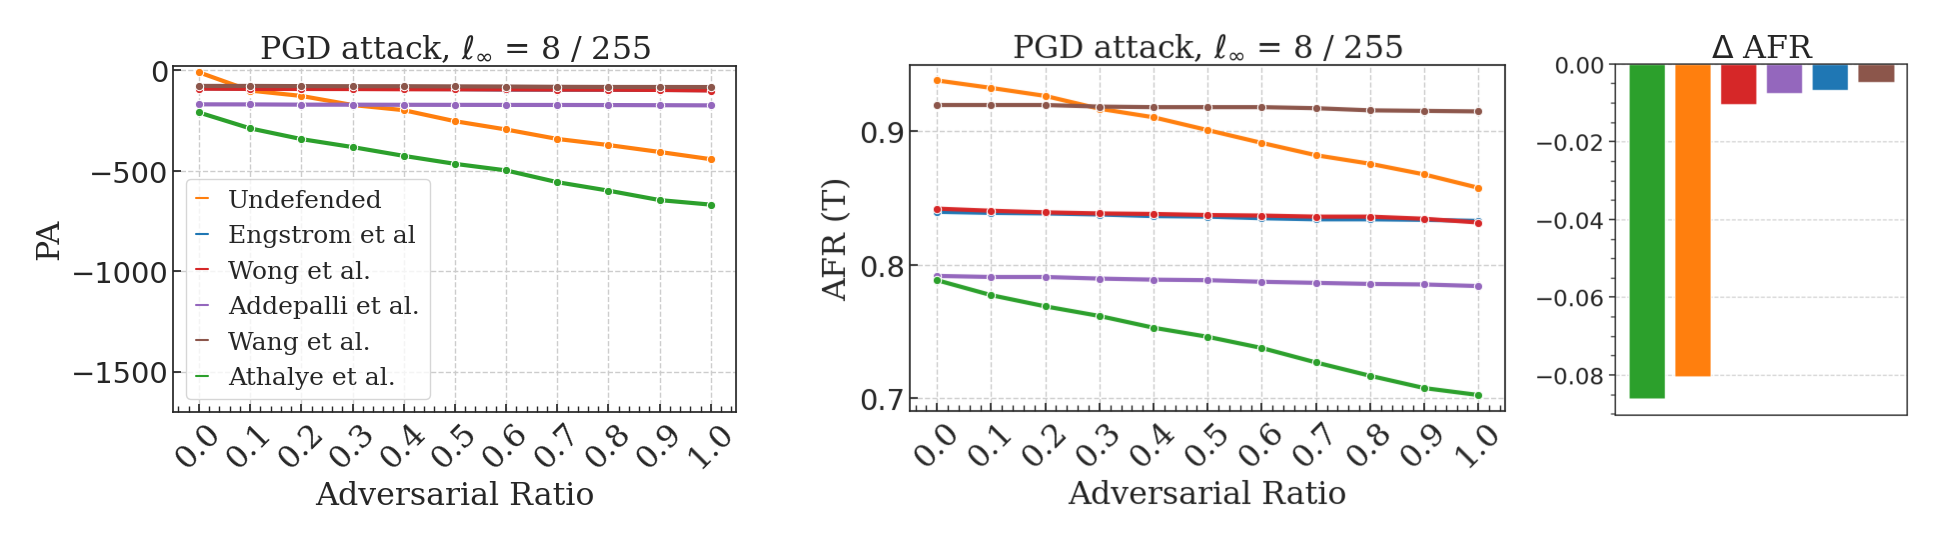
\includegraphics[width=\textwidth]{img/results_discussion/adversarial/PGD_0.0314_combo.png}
    \end{subfigure}

    \vspace{1em}

    \begin{subfigure}[b]{\textwidth}
        \centering
        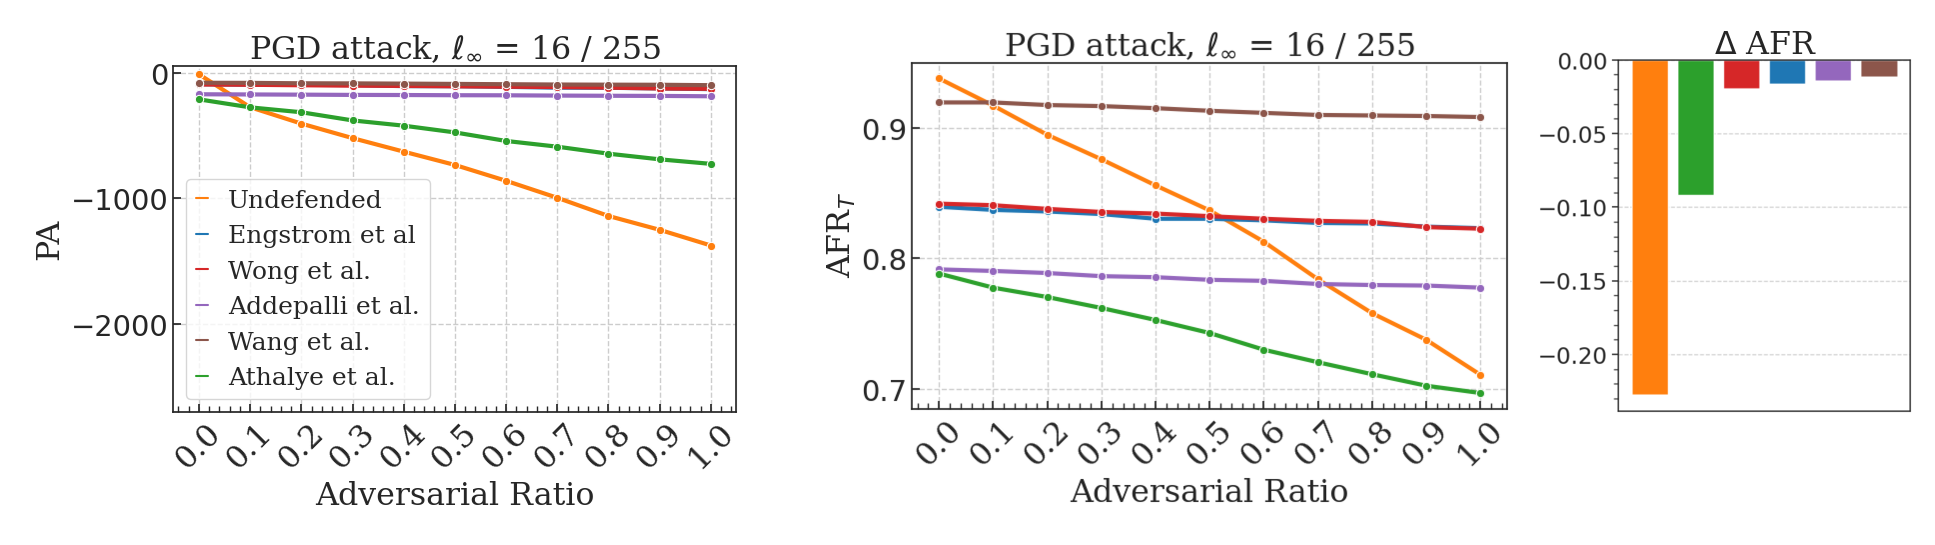
\includegraphics[width=\textwidth]{img/results_discussion/adversarial/PGD_0.0627_combo.png}
    \end{subfigure}

    \vspace{1em}

    \begin{subfigure}[b]{\textwidth}
        \centering
        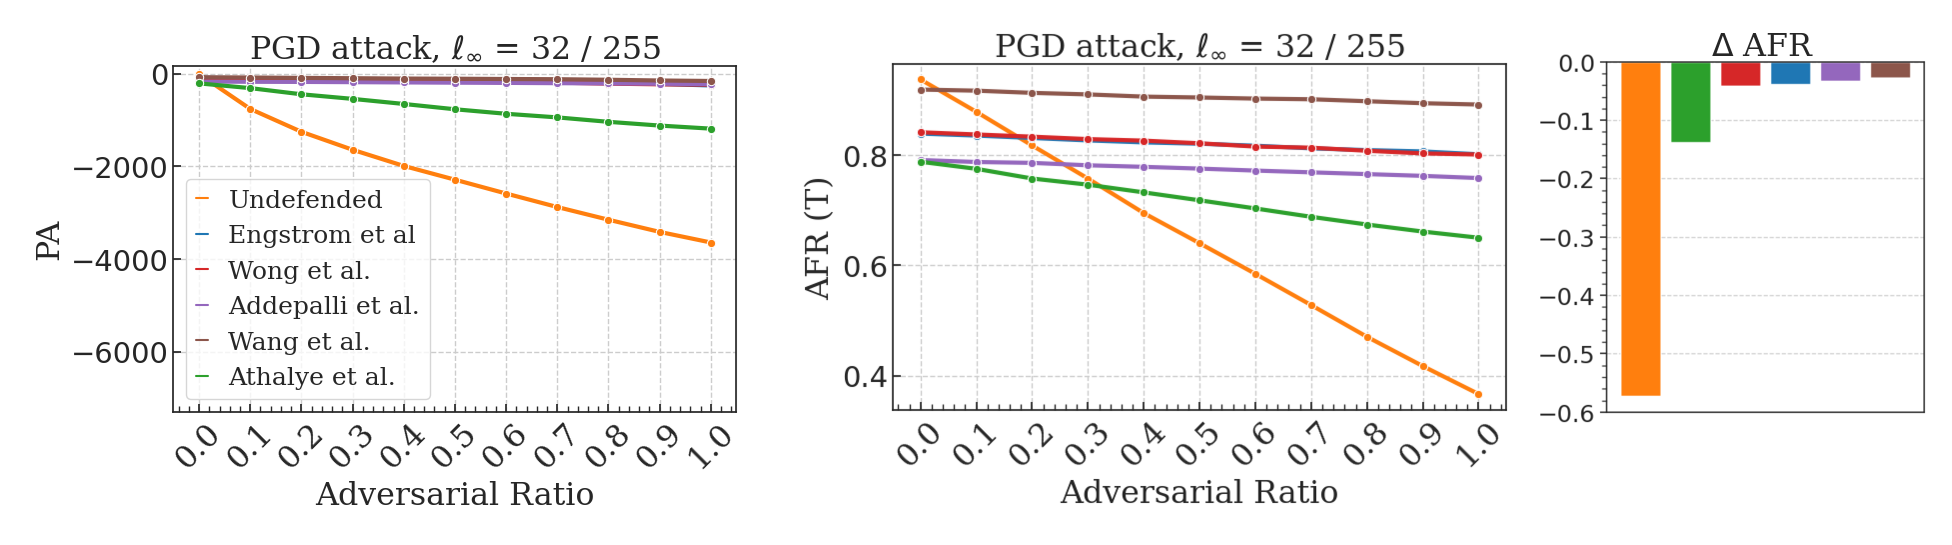
\includegraphics[width=\textwidth]{img/results_discussion/adversarial/PGD_0.1255_combo.png}
    \end{subfigure}

    \caption{PA, AFR(T) and the AFR variation against increasing adversarial ratio at different
    perturbation norm bounds. The aforementioned undefended net and several RobustBench
    robust models are considered under a 1000 step PGD attack.}
    \label{fig:six_figures_pa_adv}
\end{figure}

At first glance, it is clear that PA is able to discriminate robust models from
the {\color{tab:orange} \textbf{Undefended}} one, which is shown to significantly
decrease its performance with increasing adversarial ratio and attack power. As expected, 
the rate at which its performance decreases is higher
the more powerful the attack is, as a greater percentage of samples are able to
mislead its predictions. \\

From both PA and AFR stems the fact that {\color{tab:green} \textbf{Athalye et al.}}
is significantly less robust than its RobustBench counterparts to PGD attacks, since 
its performance decreases
way more significantly with increasing $\operatorname{AR}$. It is interesting to see, however,
than the rate at which its performance decreases is inversely proportional to the 
attack power, which indicates that the principle by which robustness is achieved
is more effective for large-norm perturbations. \\

A fundamental existing difference between these two models, that cannot be
inferred from a purely performance-based metric, is the nature of the shift in
the probabilistic output of the model, which is the source of the robust and non-robust
behaviour observed. Figure \ref{fig:unrobust_posterior_short_pgd} \textbf{(right)}
shows the optimal $\beta^{*}$ value for each model, which is an indication of
the entropy of the posterior distribution and discriminates the two non-robust
models from the rest and from each other. The {\color{tab:orange} \textbf{Undefended}}
model provides overconfident predictions that maximize disagreement in misleading and 
misclassified samples, whereas {\color{tab:green} \textbf{Athalye et al.}} provides 
uncertain predictions that minimize disagreement in adversarial samples but have 
the opposite effect in correctly classified ones. This insight clarifies the 
unintuitive behaviour observed earlier, by which {\color{tab:green} \textbf{Athalye et al.}} 
robustness value decreases at a lower rate with increasing attack power, despite maintaining a
constant decrease in performance of $\Delta \operatorname{AFR} \sim 0.1$. \\

Figure \ref{fig:unrobust_posterior_short_pgd} \textbf{(left)} illustrates
the previous reasoning by displaying the average posterior
probability assigned to the predicted class by each model, conditioned on the type
of response given by the model. This discrimination yields three groups of observations,
namely original samples that are correctly classified by the robust model, 
original samples that are misclassified and perturbed samples that, having their 
associated unperturbed sample been correctly classified, 
have been able to mislead the model. These three cases are relevant from the 
adversarial robustness perspective,  as they illustrate the trade-off between high-confident 
original predictions and adversarial vulnerability, which has been already stated in 
previous chapters. {\color{tab:brown} \textbf{Wang et al.}}
acts as a reference for an ideal robust behaviour, in which original samples are
predicted with high confidence and adversarially misleading predicted labels are 
only slightly more likely than the rest. Equivalent representations for the remaining
models can be found in Figure \ref{fig:appendix_adversarial_distribution_pgd}.\\

\begin{figure}[H]
    \centering
    \begin{subfigure}[b]{\textwidth}
        \centering
        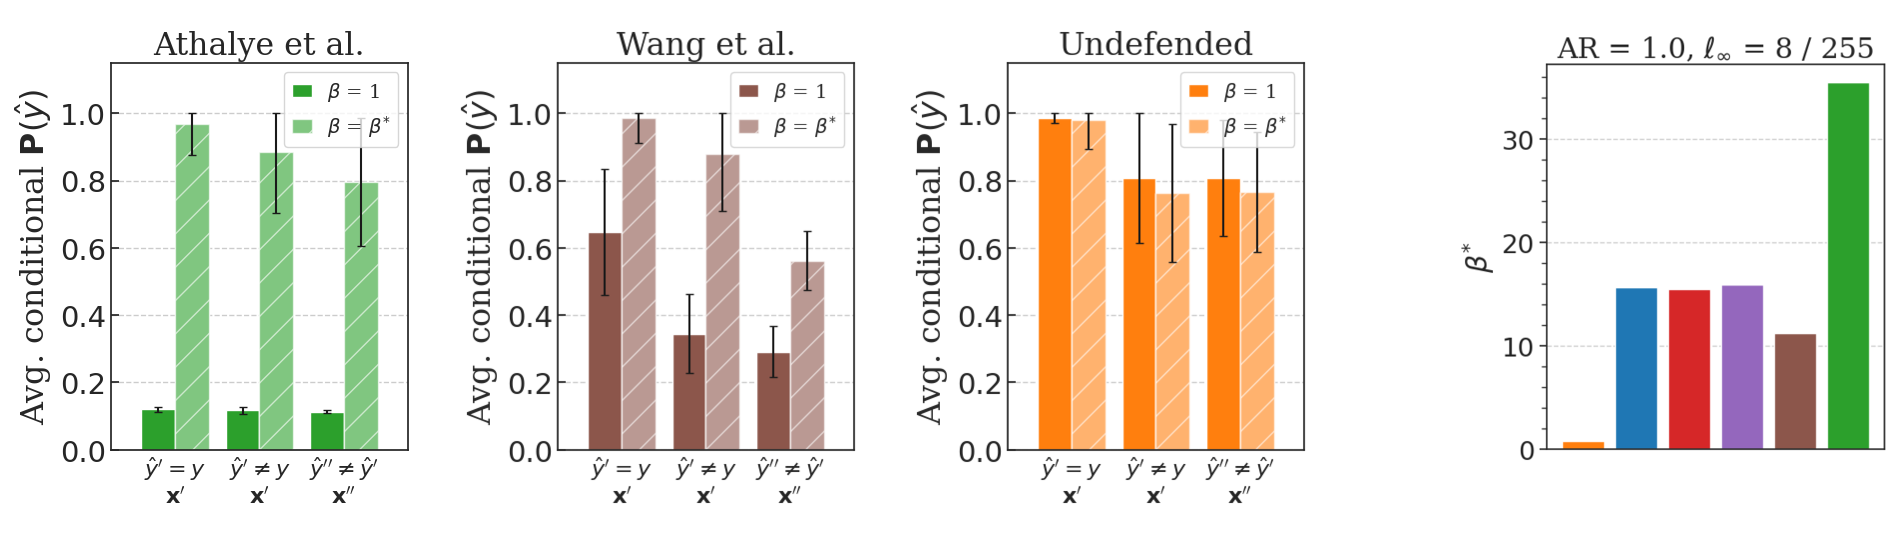
\includegraphics[width=\textwidth]{img/results_discussion/adversarial/bpda_wang_undefended_beta_pgd.png}
    \end{subfigure}
   
    \caption{(\textbf{left}) Average posterior probability of the predicted class for 
    correctly classified original samples, misclassified original samples, and 
    misleading adversarial samples, respectively. (\textbf{right}) Optimal $\beta^{*}$ value for each model.
    Results obtained through a PGD attack with $\ell_\infty = 8 / 255$.}
    \label{fig:unrobust_posterior_short_pgd}
\end{figure}

With respect to robust models, we observe a significant difference in the 
discriminative power of PA and accuracy-based metrics that does not immediately
derive from the informativeness of the optimal posterior. As remarked before, AFR (P)
constitutes our baseline robustness metric, as by definition represents the ratio
of predictions that remained constant under adversarial perturbations, and
therefore ranks models by their predictive capabilities against these attacks. The
value of $\Delta$AFR aligns with that definition, and discriminates robust models
by a very thin margin, selecting {\color{tab:brown} \textbf{Wang et al.}} as
the best. Further analysis on PA is needed to understand the source of this 
discrepancy, as for instance why {\color{tab:purple} \textbf{Addepalli et al.}} model
is attributed a significantly lower value than the remaining robust models
under a $\ell_\infty$=8/255 PGD attack, despite displaying a similar decrease in performance. \\

\begin{figure}[H]
    \centering
    \begin{subfigure}[b]{0.37\textwidth}
        \centering
        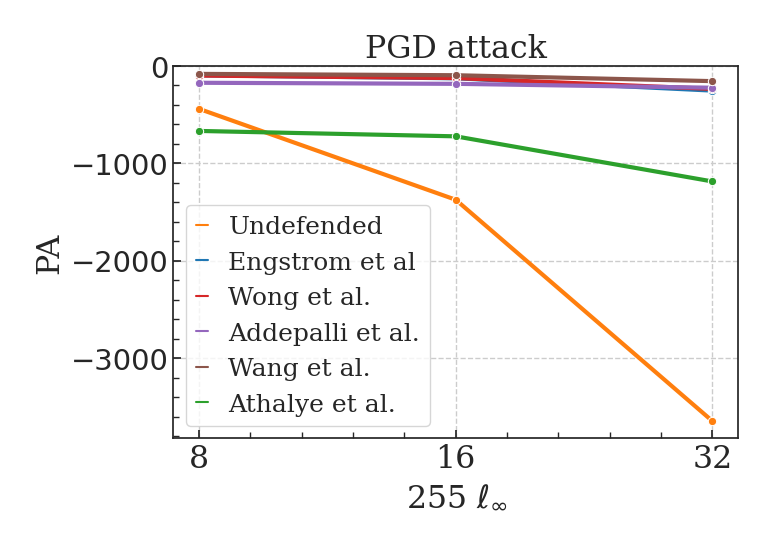
\includegraphics[width=\textwidth]{img/results_discussion/adversarial/PGD_logPA_eps.png}
    \end{subfigure}
    \hfill
    \begin{subfigure}[b]{0.59\textwidth}
        \centering
        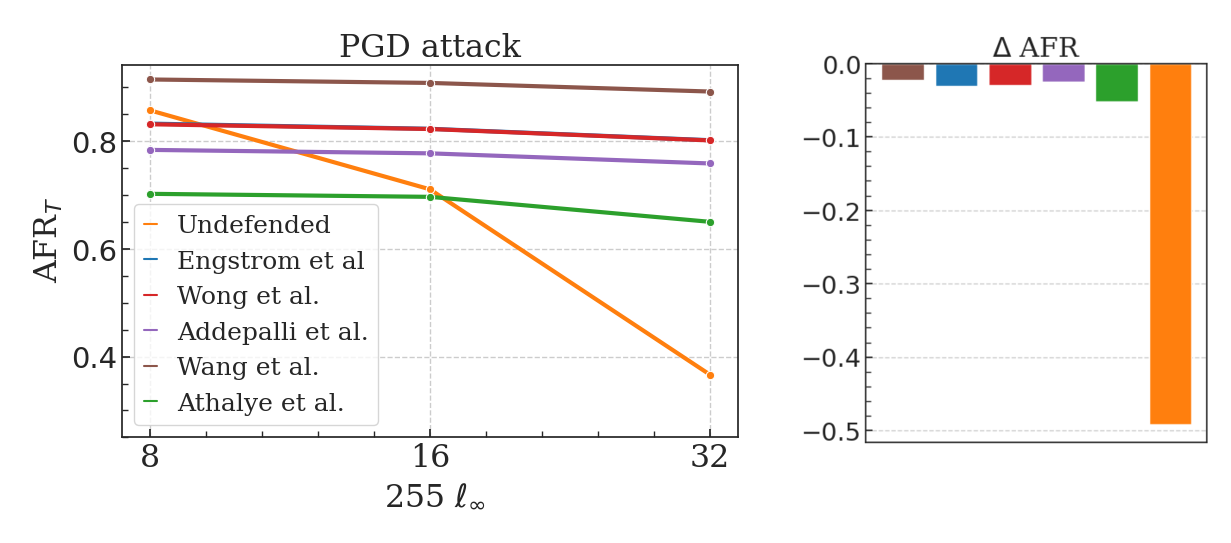
\includegraphics[width=\textwidth]{img/results_discussion/adversarial/PGD_AFR_true_eps_diff.png}
    \end{subfigure}
    \caption{PA, AFR(T) and the AFR variation against increasing attack power for  $\operatorname{AR} = 1$. 
    The aforementioned undefended net and several RobustBench robust models are considered
    under a 1000 step PGD attack.}
    \label{fig:pgd_eps}
\end{figure}

Finally, Figure \ref{fig:pgd_eps} shows that PA is also discriminative with respect to
increasing attack power, expressed through the maximum allowed $\ell_\infty$ norm. 
As mentioned earlier, PA values are heavily aligned with the performance
decrease of the models under a specific attack power, but the observed decrease in PA 
under increasing $\ell_\infty$ is much more significant that the decrease 
in performance. This can be explained by the fact that the metric is sensitive 
to the overall posterior shift and not only the position of the maximum. When increasing 
the attack power, confidence in the predicted class will decrease in general, 
even when the sample does not succeed at misleading the model, and therefore the
overall overlap between posteriors will be reduced even at comparable performance levels. \\

In order to widen the scope of the analysis, analogous results will be obtained for
a FMN attack, which is expected to be more effective than a PGD attack under 
the same conditions, given the overall decrease in $\beta^{*}$ observed 
in Table \ref{tab:entropy_gibbs}.
Figure \ref{fig:adv_fmn_pa_afr} shows the evolution of PA against 
increasing adversarial ratio for the same models, and compares
it with the assessment provided by AFR.


\begin{figure}[H]
    \centering
    \begin{subfigure}[b]{0.39\textwidth}
        \centering
        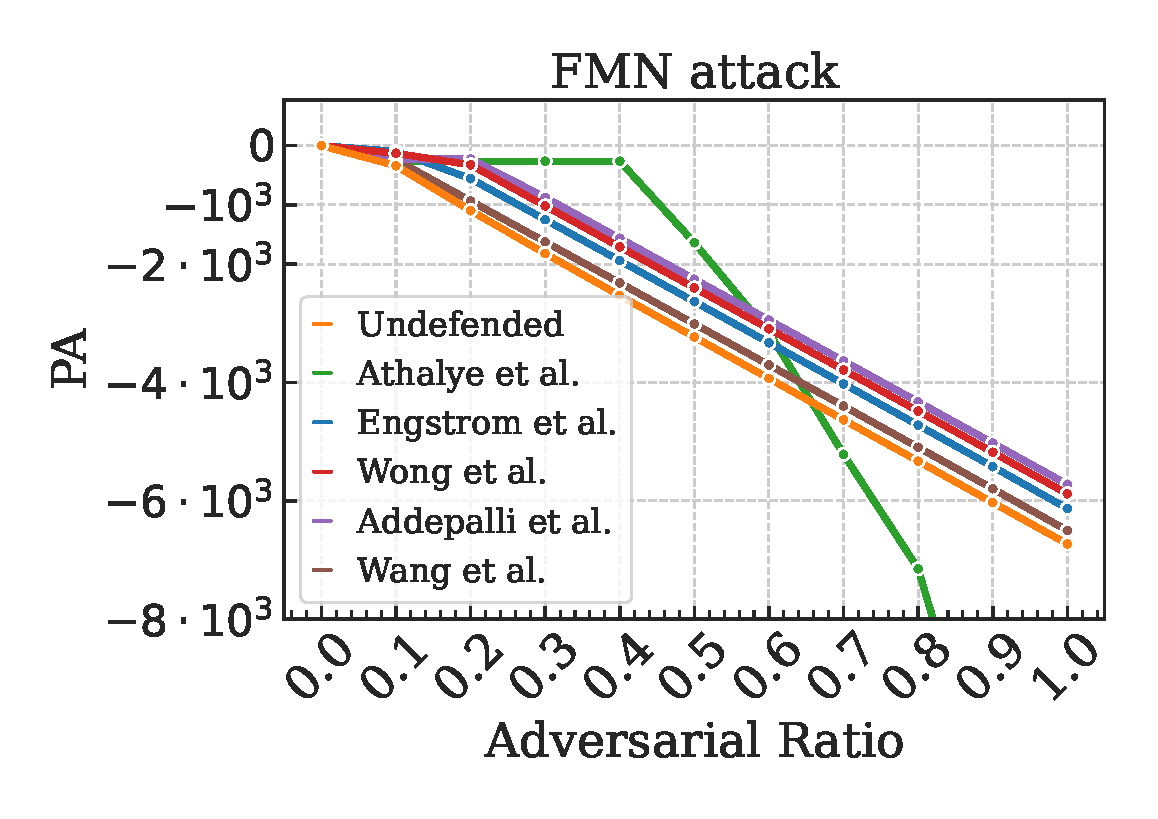
\includegraphics[width=\textwidth]{img/results_discussion/adversarial/FMN.pdf}
    \end{subfigure}
    \hfill
    \begin{subfigure}[b]{0.59\textwidth}
        \centering
        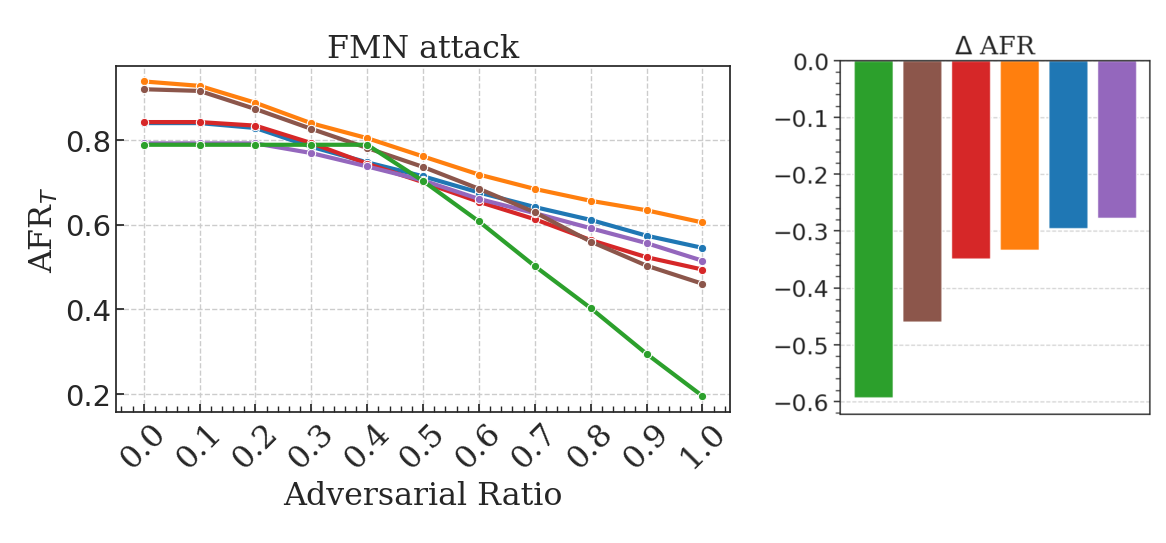
\includegraphics[width=\textwidth]{img/results_discussion/adversarial/FMN_1000_AFR_true.png}
    \end{subfigure}
    \caption{PA, AFR(T) and the AFR variation against increasing adversarial ratio. 
    The aforementioned undefended net and several RobustBench robust models are considered 
    under a 1000 step FMN attack.}
    \label{fig:adv_fmn_pa_afr}
\end{figure}


As expected, the effectiveness of the FMN attack is superior to that of PGD attacks, as
the decrease in performance is substantially more significant for all models, especially the ones
previously considered robust. It is likely that these models have been defended with a
compression strategy that succeeds at filtering out small perturbations, which are
the ones employed by FMN, and for that reason maintain their performance at low
adversarial ratio values CITE 5.
In particular, {\color{tab:green} \textbf{Athalye et al.}} remains maximally robust
until at least 40\% of the samples are perturbed, at which point the defensive strategy
is neutralized and a constant fraction of the additional perturbed samples succeeds at
misleading the model, which translates into a linear decrease in performance and PA. \\

PA proves to be very discriminative among robust models and to represent the 
phase transition entailed by the collapse of the defense strategy better than AFR does, which can be
observed in more detail in Figure \ref{fig:appendix_adversarial_afrpred_fmn}. A significative
result is that PA is not so directly aligned with $\Delta$AFR, in contrast to
the PGD case, which shows again that the decrease in performance is not the main driver of
the robustness assessment provided by PA, but instead can be interpreted as a consequence of
a misalignment in the posterior distributions of adversarial samples, which are the ones driving
the metric after the $\operatorname{AR}$ thresold is reached. \\

\begin{figure}[H]
    \centering
    \begin{subfigure}[b]{\textwidth}
        \centering
        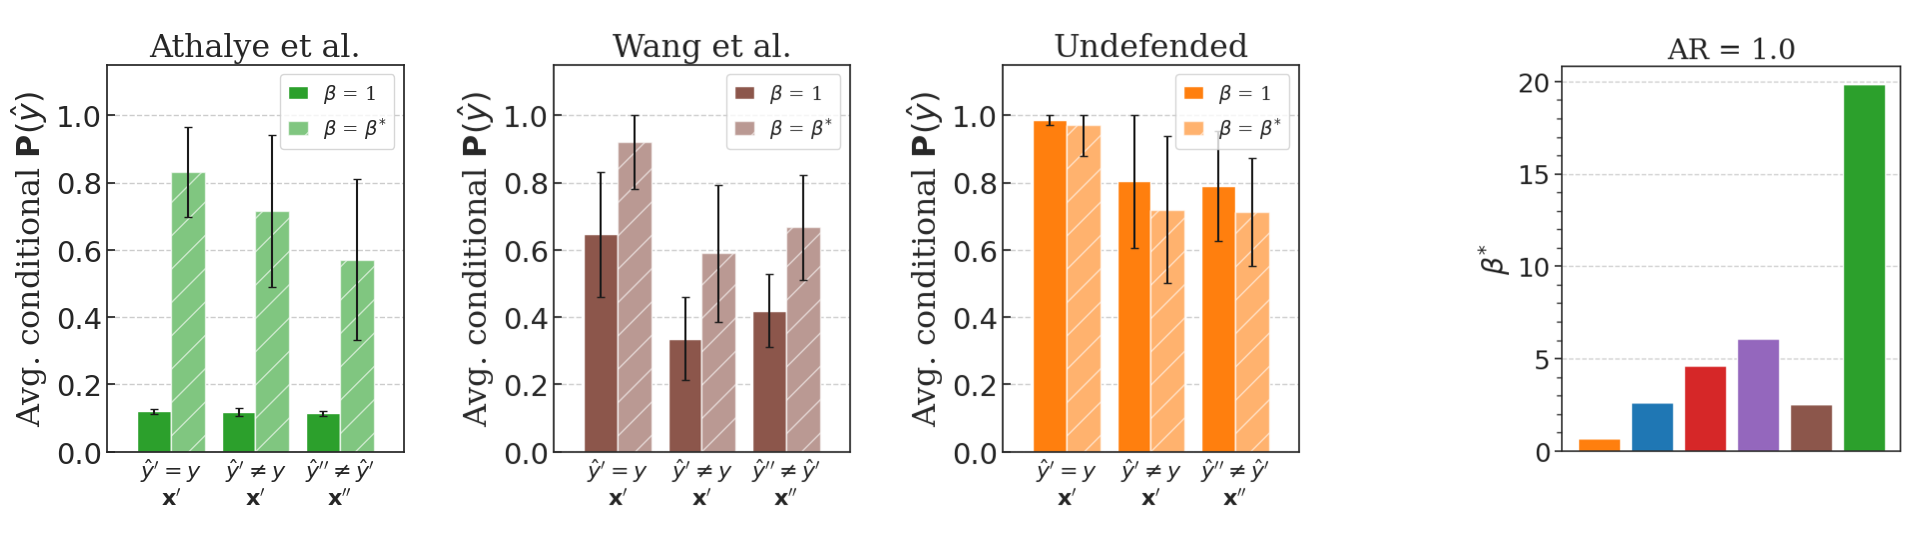
\includegraphics[width=\textwidth]{img/results_discussion/adversarial/bpda_wang_undefended_beta_fmn.png}
    \end{subfigure}
   
    \caption{(\textbf{left}) Average posterior probability of the predicted class for 
    correctly classified original samples, misclassified original samples, and 
    misleading adversarial samples, respectively. (\textbf{right}) Optimal $\beta^{*}$ value for each model.
    Results obtained through a FMN attack.}
    \label{fig:unrobust_posterior_short_fmn}
\end{figure}

Figure \ref{fig:unrobust_posterior_short_fmn} gives insight into the probabilistic output
of the model and the informativeness of the optimal posterior for the {\color{tab:orange} \textbf{Undefended}}, 
{\color{tab:green} \textbf{Athalye et al.}} and {\color{tab:brown} \textbf{Wang et al.}} models, in
analogous way to the PGD experiments. The first two models display a very similar behaviour for 
$\beta = 1$, but optimal posteriors are less informative due to the increased number of misleading
samples, which translates into a smaller $\beta^{*}$. The response of 
the {\color{tab:brown} \textbf{Wang et al.}} model further illustrates the higher effectiveness of
FMN attacks, as adversarial perturbations are on average more misleading than outlier samples in
the original dataset, which did not occur in the PGD case. Analogous representations for the remaining
models can be found in Figure \ref{fig:appendix_adversarial_distribution_fmn}, which show
that the {\color{tab:purple} \textbf{Addepalli et al.}} is the only robust model that maintains
the same behaviour under both attacks.\\

Overall, we recognize that PA has a higher discriminative power than AFR, especially
considering the evolution of each metric over increasing adversarial ratio, as
seen in Figures \ref{fig:six_figures_pa_adv} and \ref{fig:adv_fmn_pa_afr}. 
In particular, Figures \ref{fig:appendix_adversarial_afrpred_pgd} and \ref{fig:appendix_adversarial_afrpred_fmn}
compare the evolution of PA with that of AFR (P), which is the baseline metric for robustness,
and show the susceptibility of the latter to dataset variability. This is an important
consideration, as PA not only improves the discriminability in terms of the scale of
the differences between models, but also provides a more stable assessment across varying
levels of perturbed sample presence, under which AFR (P) exhibits significant fluctuations
that alter the ranking of the models at every step. \\

These observations lead to the conclusion that PA offers a more reliable
assessment of adversarial robustness, which in general aligns with the decrease
in performance on perturbed samples, but that relies heavily on the informativeness
of the posterior distribution and the confidence in the predictions for both
original and perturbed samples. \\

\subsection{Interpretability of PA in the adversarial setting}

In light of the results obtained, the suitability of
PA in the adversarial setting has been demonstrated, but a deeper exploration of the
reason of the discrepancies between PA and the baseline robustness measures is needed
so that it can confidently be established as a model selection criterion. In particular,
we will work with the approximated expression of PA derived in Theorem \ref{thm:approximated_pa} 
and ellucidate the source of the measured robust behaviour.

Table \ref{tab:approx_pa_pgd_table} shows the contribution of each subset of observations to the final
approximated PA value for a PGD attack. $N_{\text{ERR}}$, $N_{\text{MIS}}$ and $N_{\text{ADV}}$ are the number of (pairs of)
contributing samples, and $\Xi_{\text{ERR}}$, $\Xi_{\text{MIS}}$ and $\Xi_{\text{ADV}}$ are
the total amount of the contribution. For reasons described earlier in this section,
the PA approximation overestimates penalizations when compared to the true value, but
relative discrepancies between models are still largely preserved and therefore the rationale
behind the discriminative power of PA, as shown in Figures \ref{fig:appendix_adversarial_approx_pa_pgd}
and \ref{fig:appendix_adversarial_approx_pa_fmn}. The parameters $2 \delta_{\text{MIS}}$ and
$\delta_{\text{ADV}}$ account for the average probability assigned to classes other than the predicted
class for misclassified original samples and misleading adversarial samples, respectively, and 
help interpret the informativeness of the distibution as well as the value of each individual 
penalization. \\

For instance, a large $2 \delta_{\text{MIS}}$ value indicates robustness to sampling randomness, as it
represents higher average uncertainty in misclassified predictions. A model with a high performance on 
test data entails a more negative penalization $\log(1 - 2 \delta_{\text{MIS}})$, for being misclassified 
samples more likely to be equivalently misclassified under adversarial perturbations, but at
the same time makes misclassifications less likely, and therefore the number of terms added to
$\Xi_{\text{MIS}}$. The existing trade-off between standard and robust generalization arises when 
following this reasoning towards the minimization of $\Xi_{\text{MIS}}$, because reducing the number of 
misclassified samples will drive $\beta^{*}$ to higher values and therefore decrease adversarial 
uncertainty $\delta_{\text{ADV}}$. As outlined before, $\delta_{\text{ADV}}$ indicates 
robustness to adversarial perturbations, as it represents the average prediction uncertainty on adversarial 
misleading samples, and entails a penalization of $\log(\delta_{\text{ADV}})$. \\

The interpretation of these terms is vitally important for the purpose of this work, as it enables
the identification of the different sources of robustness displayed by each model, and therefore
the characterization of the randomness that we will demand models to generalize to. From a general 
perspective, $\Xi_{\text{ERR}} + \Xi_{\text{MIS}}$ can be understood as the lack of robustness
to sampling randomness, and $\Xi_{\text{ADV}}$ as the lack of robustness to adversarial perturbations. \\

\begin{table}[H]
    \centering
    \begin{tabular}{l|rr|rrr|rrr}
    Defense & $N_{\text{ERR}}$ & $\Xi_{\text{ERR}}$ & $N_{\text{MIS}}$ & $2 \delta_{\text{MIS}}$ & $\Xi_{\text{MIS}}$ & $N_{\text{ADV}}$ & $\delta_{\text{ADV}}$ & $\Xi_{\text{ADV}}$ \\
    \midrule
    {\color{tab:brown} \textbf{Wang et al.}} & 9148  & -248.38 & 799 & 0.24 & -220.24 & 47 & 0.44 & -39.44 \\
    {\color{tab:blue} \textbf{Engstrom et al.}} & 8328  & -273.26 & 1591 & 0.17 & -293.46 & 67 & 0.39 & -63.43 \\
    {\color{tab:red} \textbf{Wong et al.}} & 8329  & -254.37 & 1562 & 0.17 & -282.88 & 90 & 0.38 & -88.98 \\
    {\color{tab:purple} \textbf{Addepalli et al.}} & 7840  & -390.25 & 2063 & 0.21 & -487.17 & 75 & 0.46 & -58.92 \\
    {\color{tab:orange} \textbf{Undefended}} & 8569  & -372.49 & 566 & 0.47 & -364.14 & 810 & 0.24 & -1173.55 \\
    {\color{tab:green} \textbf{Athalye et al.}} & 7136 & -458.39 & 1915 & 0.23 & -505.46 & 747 & 0.21 & -1183.96 \\
    \bottomrule
    \end{tabular}
    \caption{
    Approximated PA contributions for a PGD attack with $\ell_\infty$ = 8/255 and 
    $\operatorname{AR} = 1.0$. The number of contributing samples for each term is 
    $N_{\text{ERR}} = \lfloor N \tau \rho \rfloor$, $N_{\text{MIS}} = \lfloor N (1-\tau) \rho \rfloor$ and
    $N_{\text{ADV}} = \lfloor N \tau (1-\rho) \rfloor$. The penalization argument $2 \delta_{\text{ERR}}$ has not
    been included for being negligible in all cases.
    }
    \label{tab:approx_pa_pgd_table}
\end{table}

- $\Xi_{\text{ERR}}$ aligns perfectly with AFR(T) at AR=1, given that penalization terms are 
similar for being beta quite high.\\
- $\Xi_{\text{MIS}}$ adds to this penalization but in a much more non-linear way, and illustrate
the trade-off described before, by which models containing less correct observations have smaller
penalization terms (larger dmis, see athalye), but more samples contributing, which adds up
to a higher total penalization. In the absence of adversarial samples, these models would be the most
robust. Undefended > Addepalli > Athalye.\\

- $\Xi_{\text{ADV}}$ is the least discriminative term, which makes sense given the small effectivity
of the attack. The $\Xi_{\text{ADV}}$ is driven by the decrease in performance beacuse its the number
of terms Nadv, but its modulated by the penalization term derived from dadv. This amounts to
the general interpretation of the PA kernel, which is equivalent to accuracy but instead of adding 
binary penalizations it contributes with a negative penalization term in the range [-inty, 0].\\

THIS SHOULD BE IN THE END.
- When we sum these contributions, we lose the direct dependency on AFR(T) and Delta AFR, because
we aggregate the robustness penalization contributed by the two sources of robustness. \\
This is a very important realization, as we show that PA provides a unified approach to robust model
selection, that unifies sampling randomness and adversarial randomness into a single
value. A weighted metric between AFR(T) and DeltaAFR (or AFR (T)) would be completely arbitrary
and would not adjust to the particularities of each model output. For instance, Undefended should be
penalized for its lack of robustness to adversarial examples, whereas Athalye should be penalized
for its lack of robustness to adversarial perturbations. PA provides a unified way of doing that
based on the whole probability distribution and therefore 


The values displayed on the tables cannot be compared in between attacks, as they are tied
to a specific value of $\beta^{*}$. 

\begin{table}[h]
    \centering
    \begin{tabular}{l|rr|rrr|rrr}
    Defense & $N_{\text{ERR}}$ & $\Xi_{\text{ERR}}$ & $N_{\text{MIS}}$ & $2 \delta_{\text{MIS}}$ & $\Xi_{\text{MIS}}$ & $N_{\text{ADV}}$ & $\delta_{\text{ADV}}$ & $\Xi_{\text{ADV}}$ \\
    \midrule
    {\color{tab:purple} \textbf{Addepalli et al.}} & 2864 & -401.85 & 753 & 0.52 & -553.50 & 1093 & 0.28 & -1394.45 \\
    {\color{tab:orange} \textbf{Undefended}} & 3123 & -182.56 & 206 & 0.56 & -169.73 & 1566 & 0.29 & -1953.27 \\
    {\color{tab:red} \textbf{Wong et al.}} & 2749 & -243.81 & 516 & 0.46 & -318.95 & 1460 & 0.27 & -1922.20 \\
    {\color{tab:blue} \textbf{Engstrom et al.}} & 2945 & -525.45 & 562 & 0.72 & -709.37 & 1252 & 0.32 & -1424.00 \\
    {\color{tab:brown} \textbf{Wang et al.}} & 2490 & -424.24 & 217 & 0.82 & -375.30 & 2107 & 0.33 & -2318.73 \\
    {\color{tab:green} \textbf{Athalye et al.}} & 1602 & -665.08 & 429 & 0.57 & -362.03 & 2339 & 0.43 & -1977.71 \\
    \bottomrule
    \end{tabular}
    \caption{
    Approximated PA contributions for a FMN attack with 
    $\operatorname{AR} = 1.0$. The number of contributing samples for each term is 
    $N_{\text{ERR}} = \lfloor N \tau \rho \rfloor$, $N_{\text{MIS}} = \lfloor N (1-\tau) \rho \rfloor$ and
    $N_{\text{ADV}} = \lfloor N \tau (1-\rho) \rfloor$. The penalization argument $2 \delta_{\text{ERR}}$ has not
    been included for being negligible in all cases, with the exception of {\color{tab:green} \textbf{Athalye et al.}}, in which 
    it amounts to $0.36$ and explains the large value of $\Xi_{\text{ERR}}$.
    }
    \label{tab:approx_pa_fmn_table}
\end{table}

This expression allows us to interpret the results of PA in the adversarial setting. For instance,
we expect a baseline PA value at $\operatorname{AR} = 0.0$q  driven by the accuracy of the model



Even if the ultimate 


Both models 
Given the shape of the posterior, mismatched samples will be
highly pena\\

AFTER THE PLOT OF THE TWO.

The ideal is to maximize confidence on true samples, keeping high accuracy, 
and minimize confidence in adversarial samples. If standard performance is significantly high,
then optimal beta will be lower the higher is the confidence in correctly classified original samples.
If, at the same time, the confidence in misleading samples is low, the gibbs posterior will be small
and therefore the penalization will be reduced. 

That's why PA behaves as an intermediate between a performance metric and a robustness metric,
in the sense that PA penalization terms will be lower the lower is the confidence in
adversarially misleading prediction, but at the same t

Given the non-linearity of the logarithm in
the interval $[0,1]$, the second option is b
optimal posterior for adversarial samples will not be very hig


\
 arises due to overfitting to the data, and results in a model that
not


This
results in a very low optimal $\beta$ value, as shown in Figure \ref{fig:unrobust_posterior_short} (\textbf{right}),




Both models show an opposite behaviour regarding their predictive outcome,

These results illustrate the prediction 



as per the robustness trade-off
mentioned in previous chapters, a

Once the source of discrimination between the {\color{tab:orange} \textbf{Undefended}} and
{\color{tab:green} \textbf{Athalye et al.}} models has been established, we can proceed 
with the exploration of the discrimination established between the {\color{tab:purple} \textbf{Addepalli et al.}}
model and the remaining robust models, which is maximum for $\ell_\infty = 8 / 255$ and
vanishes for $\ell_\infty = 32 / 255$. \\


WHEN YOU SHOW THE PLOTS: EXPLAIN THE REASON BEHIND LINEAR BEHAVIOUR, ETC...
(see ).

he value of $\Delta$ AFR aligns
with that of AFR(P), and obviously succeeds at discriminating 

$\Delta$ AFR is
the baseline robustness metric, as it represents t

as the model is not able to maintain its predictive

which in these experiments correspond to the  and 
{\color{tab:green} \textbf{Athalye et al.}} cases. This is clear from the fact that these
two models 


These results show that PA is consistently discriminating 

As we can see, PA consistently discriminates between the twho models over increasing
attack power.

- The undefended model shows the vulnerability of accuracy, because there is no regularization (defense) that makes a specific region in the latent space around the original sample that makes the model yield the same prediction. Even if the performance of the model is higher than that of robust models for low AR values, the Undefended model is clearly less robust, and only PA is able to account for that.
- The rest of the models only decrease slightly in performance with increasing shift ratio, because most of perturbed predictions yield the same result. In that sense, all models achieve similar levels of robustness. PA clearly distinguishes those two groups.

We would like to know where does this discrimination stem from, and for that we will have to dive deeper into the predictions yielded by the different models.


- To begin with, we can compare how does PA adjust to the actual measurement of robustness as per the classical definition in the adversarial setting. Looking at the results, we see that the principal driver of the discrimination in PA can be explained by the accuracy decrease between models. As expected, AFR (P) represents the classical definition of robustness, as its value is driven by the ratio of performance decrease.
- Some examples that we will consider:
    - Difference between the robust group vs the non-robust group (BPDA and Standard):
        - We can see that this distinction is made clear in both AFR and PA. Both models are less robust in 8/255 because their performance drops with increasing adversarial ratio, indicating that advesarial samples are able to mislead the model significantly. This distinction is seen more clearly in the optimal beta values, as BPDA and Undefended are clear outliers.
        - Posterior agreement discriminates models better, and aligns more with the expected linear decay of robustness over linear incremental adversarial ratio.
    - Difference between non-robust (BPDA and Standard)
        - At 8/255 we have almost same robustness, because accuracy slopes decrease at the same rate in AFR(T), and at 32/255 we have BPDA gains robustness. This is better seen in the DeltaAFR plot, as it represents the classical robustness metric **baseline**.
        - Both models are discriminated by the beta value, but we see that they are outliers in different directions. This indicates a fundamental difference in the robustness expression that will also be important to understand the discrimination made from Addepalli and the rest.
        - There is an intrinsic difference between distributions in the BPDA case and the Standard case. This is only distinguished by PA. First, because its evolution (decrease rate) is aligned with the observed robustness baseline. But also because the predictive behaviour of both models is intrinsically different, and that can only be seen using BETA. Maybe show the beta plot. CONSIDER ADDING THE BETA PLOT IN THE THEORY, AND THEN REFERENCE IT HERE.
            - [REFERENCE TO BETA PLOT]
- Regarding PA, we see nevertheless that the discriminative power is driven by something additional, that does not vary in between positive ARs for the robust models, and that allows us to discriminate Wang et al. (purple) from the other robust models when epsilon is small, and also BPDA from Standard for 8/255, even if both models present a similar decrease in performance.  In order to ellucidate that, we have to take a direct look to the model’s predictions.
    - [PLOT]: Relationship between prediction confidence and beta when AR=0.0. All three models have comparable performances, but their predictive output is completely different. This plot illustrates the meaning behind the value of optimal beta.


\begin{figure}[H]
    \centering
    \begin{subfigure}[b]{0.3\textwidth}
        \centering
        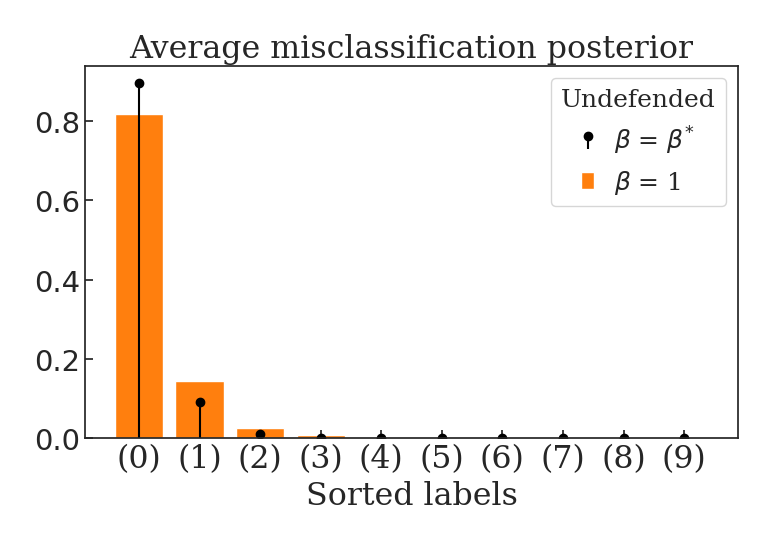
\includegraphics[width=\textwidth]{img/results_discussion/adversarial/PGD_0.0314_probability_misclass_standard.png}
    \end{subfigure}
    \hfill
    \begin{subfigure}[b]{0.3\textwidth}
        \centering
        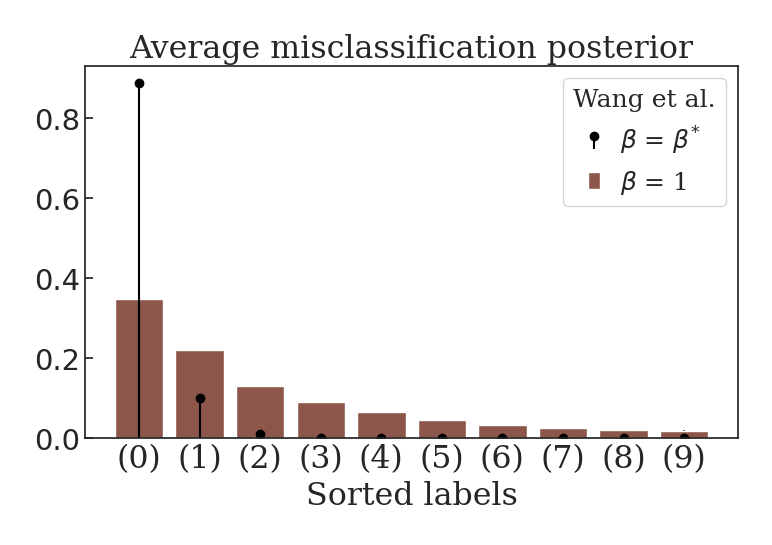
\includegraphics[width=\textwidth]{img/results_discussion/adversarial/PGD_0.0314_probability_misclass_wang2023.png}
    \end{subfigure}
    \hfill
    \begin{subfigure}[b]{0.3\textwidth}
        \centering
        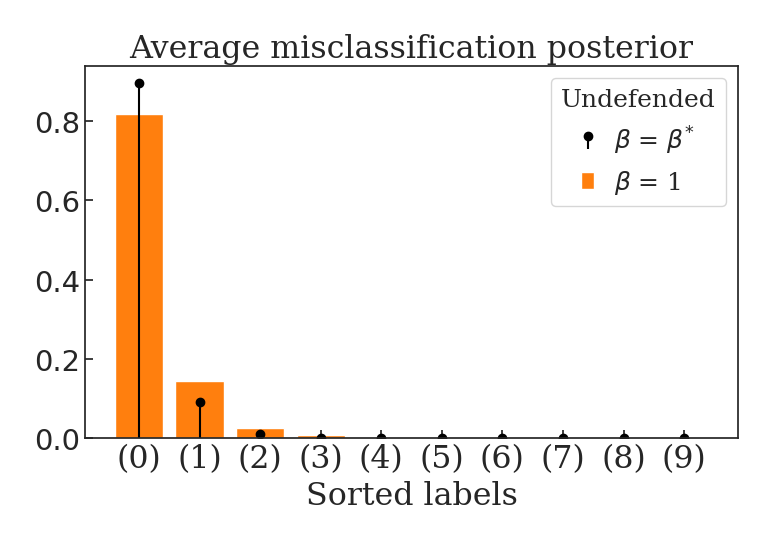
\includegraphics[width=\textwidth]{img/results_discussion/adversarial/PGD_0.0314_probability_misclass_standard.png}
    \end{subfigure}
    \caption{Relationship between prediction confidence and beta when AR=0.0. All three models have comparable performances, but their predictive output is completely different. This plot illustrates the meaning behind the value of optimal beta.}
\end{figure}

- It is worth noting that this is a 10-class classification problem, and we expect wrong predictions in the original dataset to have a more flattened distribution than correct predictions. For that reason, we expect PA to penalize disagreement over correct predictions than over incorrect predictions, and therefore to be more highly correlated with the true performance AFR (T) than with the actual robustness in the classical sense AFR (P). We can see this below.



AR=1.0. We can explain the posterior agreement values by looking at this plot, which represents the difference between the probability assigned to the highest confidence prediction for true, original samples and false, adversarial samples. As we can see, some models yield a higher confidence to the right class, nevertheless still yield high confidence to the wrong adversarial predicted class. Balance between low adversarial probability and wide gap between original true and adv false. ONLY ONE OF THEM IS ENOUGH

\begin{figure}[H]
    \centering
    \begin{subfigure}[b]{0.49\textwidth}
        \centering
        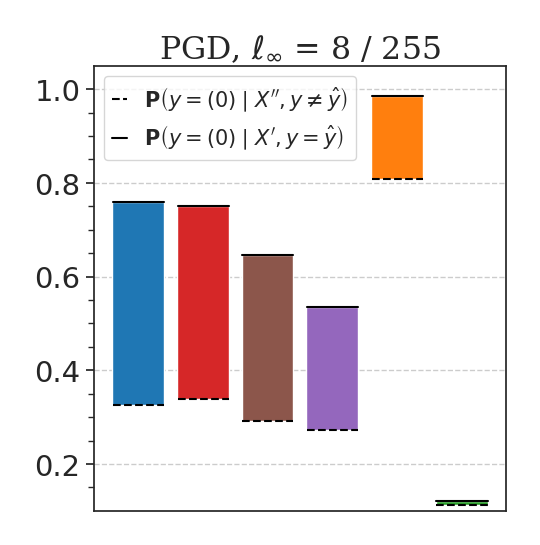
\includegraphics[width=\textwidth]{img/results_discussion/adversarial/DIFF_PGD_0.0314.png}
    \end{subfigure}
    \hfill
    \begin{subfigure}[b]{0.49\textwidth}
        \centering
        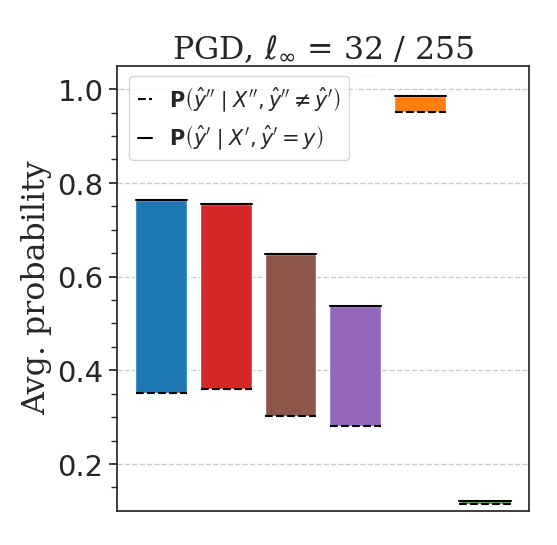
\includegraphics[width=\textwidth]{img/results_discussion/adversarial/DIFF_PGD_0.1255.png}
    \end{subfigure}
    \caption{Difference.}
    \label{fig:gaussian_optimization}
\end{figure}


Also works with FMN:
- Posterior agreement discriminates models in a different way as does AFR.
- Now we observe a great decrease of PA under increasing shift ratio.
- FMN is way more effective at decreasing accuracy.


- We can compare with PGD:
    - Original accuracy is the same because models are the same.
    - In all ROBUST models, FMN attacks are more successful because, on average, a higher confidence is given to adversarial misleading examples. The non-robust model behaves similarly, and the accuracy drop (see before) is also similar.
    - FMN attacks are more successful in RED than BLUE, as the accuracy drop is larger and the

\begin{figure}[H]
    \centering
    \begin{subfigure}[b]{0.49\textwidth}
        \centering
        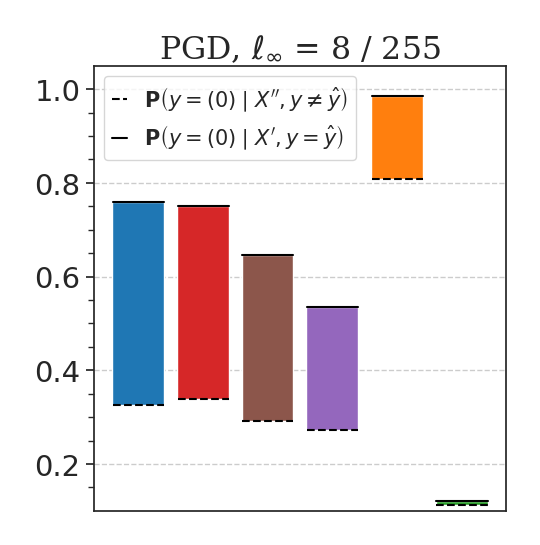
\includegraphics[width=\textwidth]{img/results_discussion/adversarial/DIFF_PGD_0.0314.png}
    \end{subfigure}
    \hfill
    \begin{subfigure}[b]{0.49\textwidth}
        \centering
        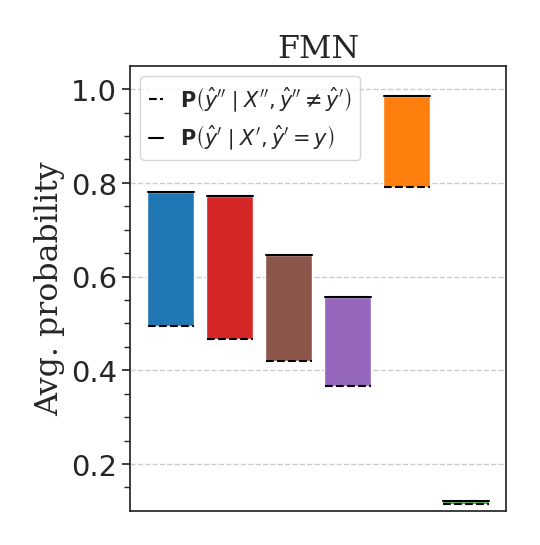
\includegraphics[width=\textwidth]{img/results_discussion/adversarial/DIFF_FMN.png}
    \end{subfigure}
    \caption{Difference.}
    \label{fig:gaussian_optimization}
\end{figure}


PROOF: Wasserstein and KL.

- An aggregated similarity measure between distributions is very informative but it does not correctly predict robustness in the outcome, as it treats all labels equally. This means that there is no penalization for disagreement or agreement, which is key for robustness assessment. For instance, BPDA is not penalized for having a flat distribution.

\begin{figure}[H]
    \centering
    \begin{subfigure}[b]{0.45\textwidth}
        \centering
        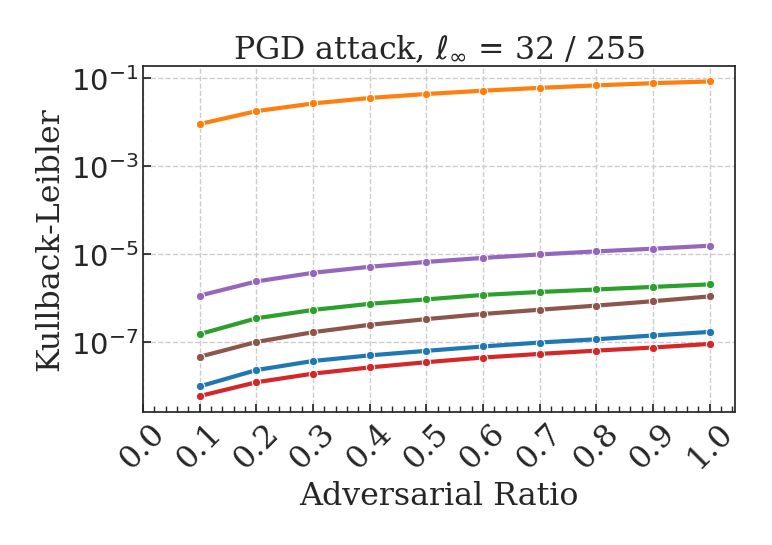
\includegraphics[width=\textwidth]{img/results_discussion/adversarial/PGD_KL.png}
    \end{subfigure}
    \hfill
    \begin{subfigure}[b]{0.45\textwidth}
        \centering
        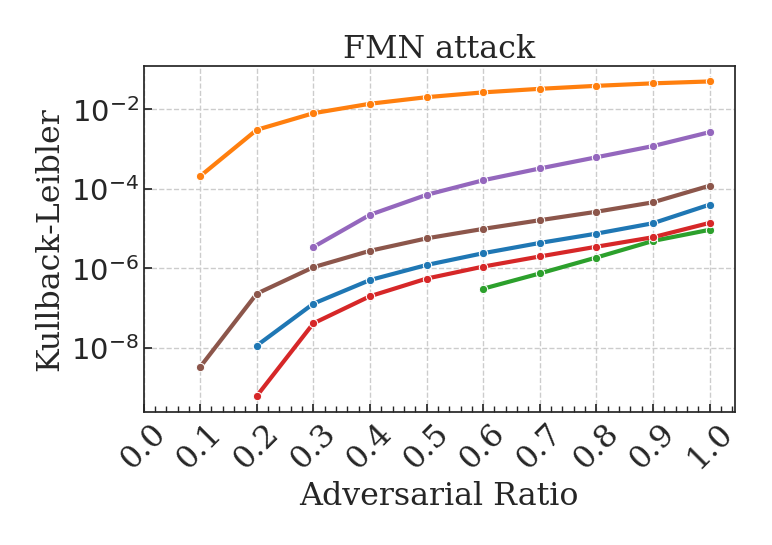
\includegraphics[width=\textwidth]{img/results_discussion/adversarial/FMN_KL.png}
    \end{subfigure}

    \vspace{1em}

    \begin{subfigure}[b]{0.45\textwidth}
        \centering
        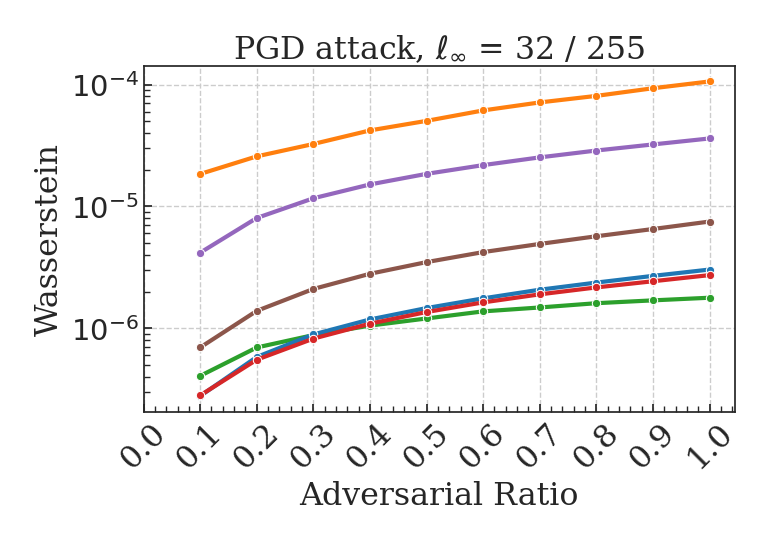
\includegraphics[width=\textwidth]{img/results_discussion/adversarial/PGD_W.png}
    \end{subfigure}
    \hfill
    \begin{subfigure}[b]{0.45\textwidth}
        \centering
        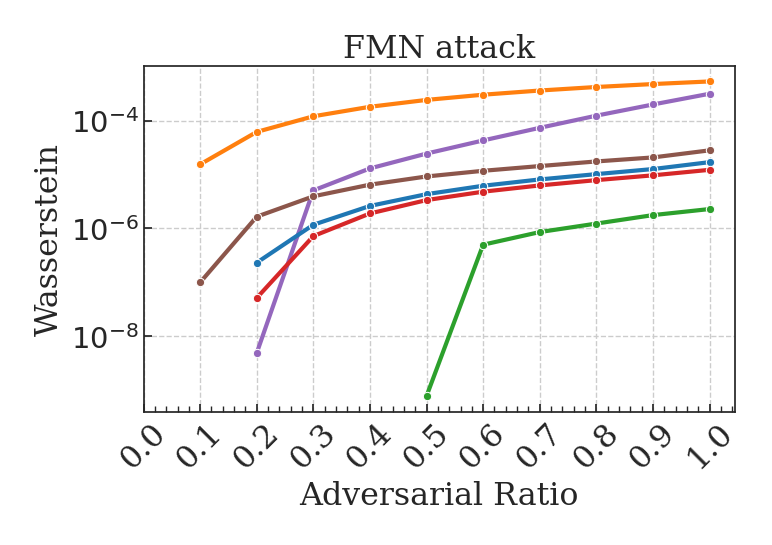
\includegraphics[width=\textwidth]{img/results_discussion/adversarial/FMN_W.png}
    \end{subfigure}

    \caption{Comparison using probability based distances.}
    \label{fig:six_figures}
\end{figure}

- As an alternative to posterior agreement we can try to infer robustness from the feature space (add here the right notation).
- For the FMN case they are not discriminative until a sufficiently high AR is achieved. Only when adversarial samples are labeled as such we could use these metrics (similar to anomaly detection) to assess similarity, but they would still be less informative about the feature space.

\begin{figure}[H]
    \centering
    \begin{subfigure}[b]{0.45\textwidth}
        \centering
        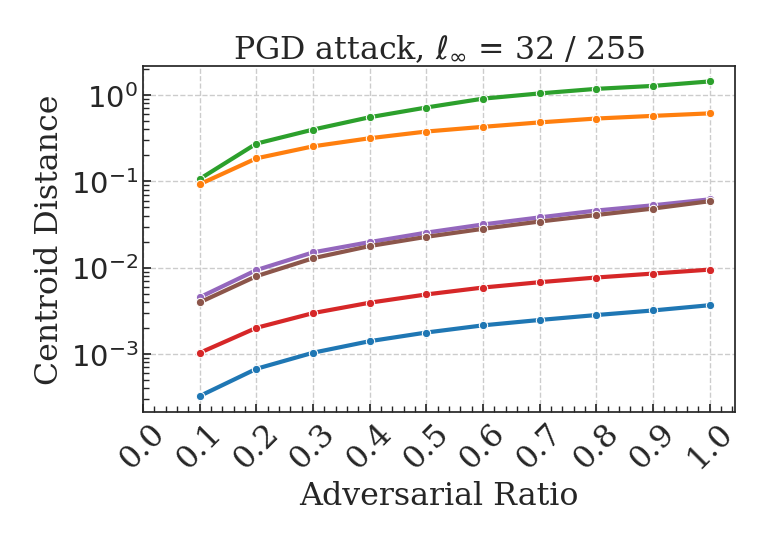
\includegraphics[width=\textwidth]{img/results_discussion/adversarial/PGD_CD.png}
    \end{subfigure}
    \hfill
    \begin{subfigure}[b]{0.45\textwidth}
        \centering
        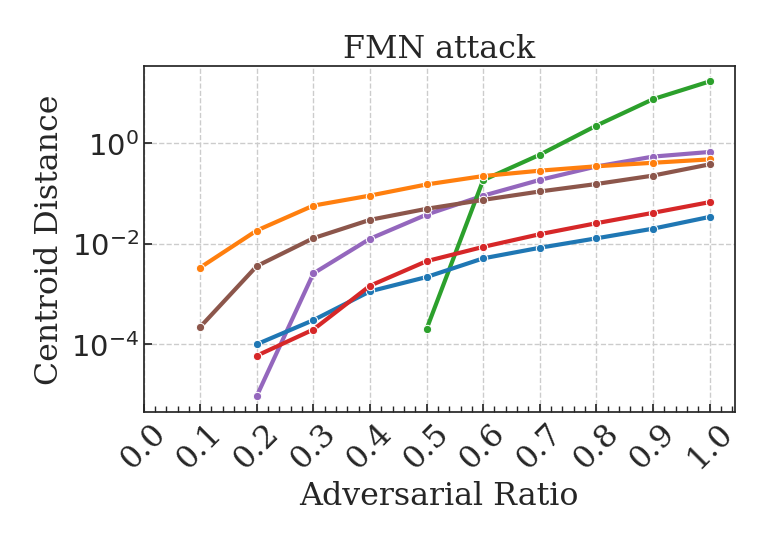
\includegraphics[width=\textwidth]{img/results_discussion/adversarial/FMN_CD.png}
    \end{subfigure}

    \vspace{1em}

    \begin{subfigure}[b]{0.45\textwidth}
        \centering
        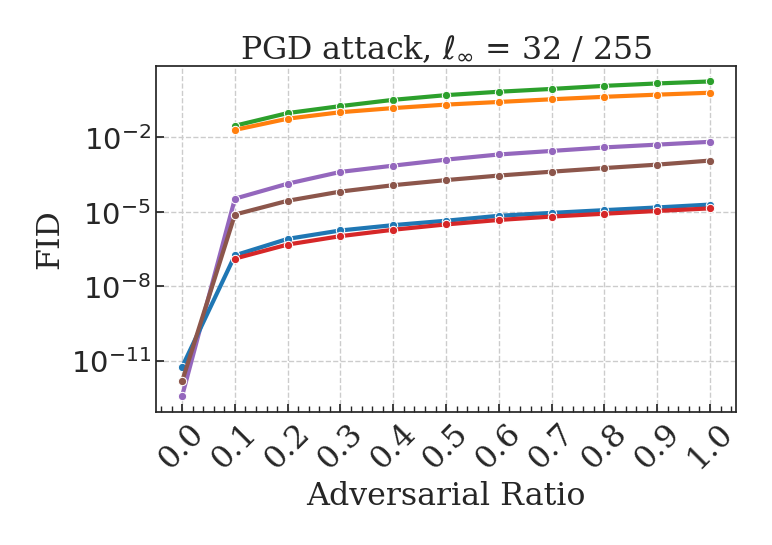
\includegraphics[width=\textwidth]{img/results_discussion/adversarial/PGD_FID.png}
    \end{subfigure}
    \hfill
    \begin{subfigure}[b]{0.45\textwidth}
        \centering
        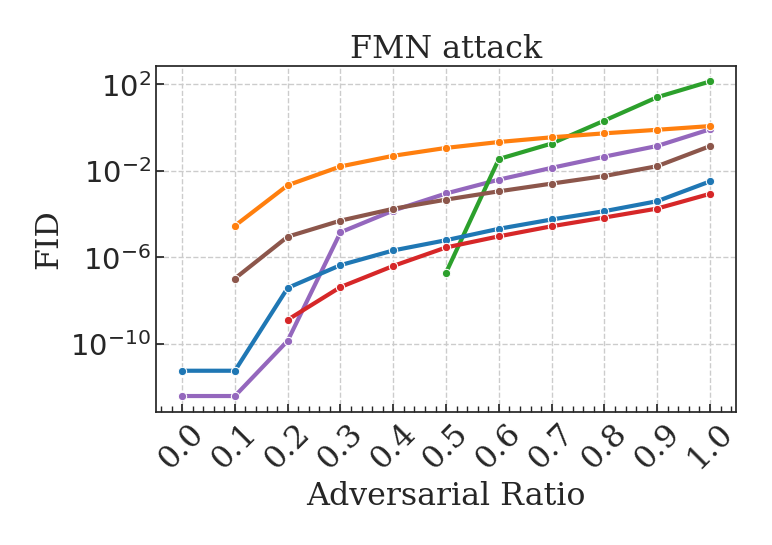
\includegraphics[width=\textwidth]{img/results_discussion/adversarial/FMN_FID.png}
    \end{subfigure}

    \caption{Comparison using feature-space based distances.}
    \label{fig:six_figures}
\end{figure}



CLAIM: Robustness against increasing attack power

PROOF: Following plots. PA decreases with increasing attack power at AR=1.0.

- Only PA clearly discriminates BPDA from the rest of robust models. As explained before, this discrimination is fundamental and will be highly value in the domain generalization setting.
- The classical robustness definition discriminates the standard from the rest, as seen in DeltaAFR.
- For the reasons given before (peaked posterior distribution at betamax, etc), logPA is able to replicate the AFR (T) response.
- Feature space metrics show a constant increase of the distance between X and Xprime representations. The only model that does not follow the same trend is Standard, indicating that the feature space is not able to represent the shift represented by adversarial features.
- Posterior distance metrics discriminate also BPDA. In general, over increasing attack power, we see that feature-space and distribution-based distance metrics tend to behave differently. In all cases, they overfit to the increased distance existing between true and adversarial predictions in the red,blue model.



\begin{figure}[H]
    \centering
    \begin{subfigure}[b]{0.22\textwidth}
        \centering
        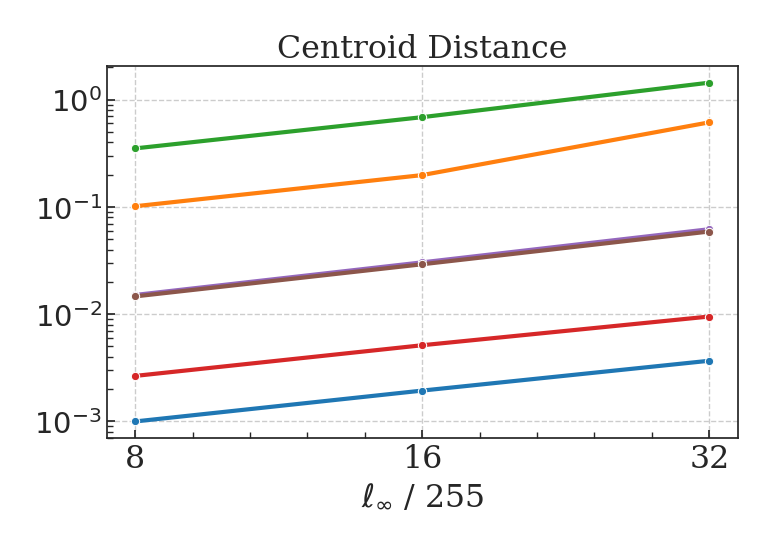
\includegraphics[width=\textwidth]{img/results_discussion/adversarial/PGD_CD_eps.png}
    \end{subfigure}
    \hfill
    \begin{subfigure}[b]{0.22\textwidth}
        \centering
        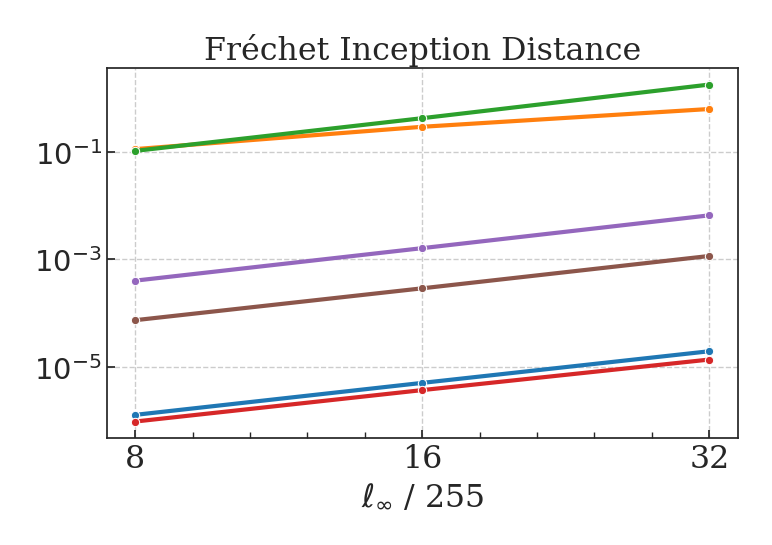
\includegraphics[width=\textwidth]{img/results_discussion/adversarial/PGD_FID_eps.png}
    \end{subfigure}
    \hfill
    \begin{subfigure}[b]{0.22\textwidth}
        \centering
        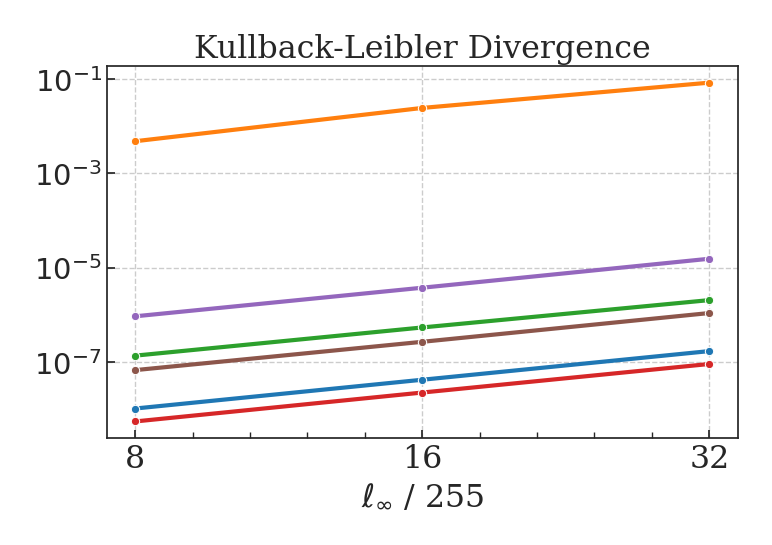
\includegraphics[width=\textwidth]{img/results_discussion/adversarial/PGD_KL_eps.png}
    \end{subfigure}
    \hfill
    \begin{subfigure}[b]{0.22\textwidth}
        \centering
        \vspace{-5pt}
        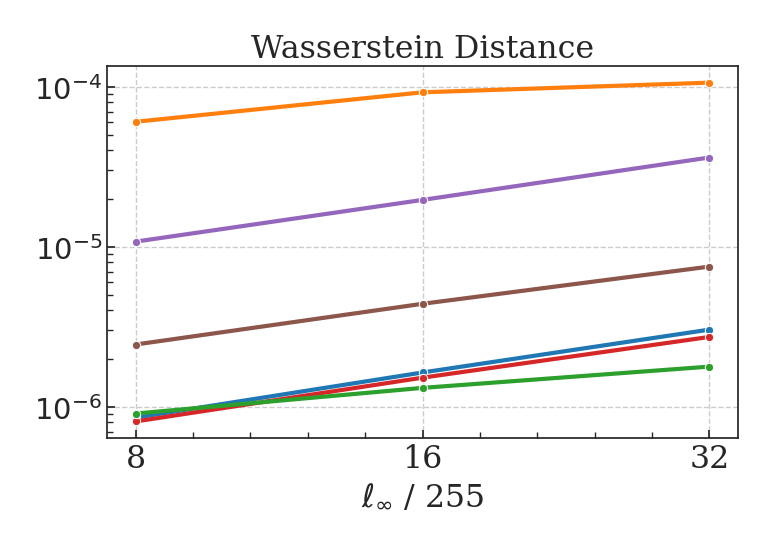
\includegraphics[width=\textwidth]{img/results_discussion/adversarial/PGD_W_eps.png}
    \end{subfigure}
    \caption{How metrics evolve with eps.}
    \label{fig:gaussian_optimization}
\end{figure}

This can be observed even more clearly on the gaussian attack. Both PA and AFR are able to select the Undefended model as the least robust one, in the sense that their predictions suffer greater change with increasing attack power. Nevertheless, PA is much more discriminative than

\begin{figure}[H]
    \centering
    \begin{subfigure}[b]{0.3\textwidth}
        \centering
        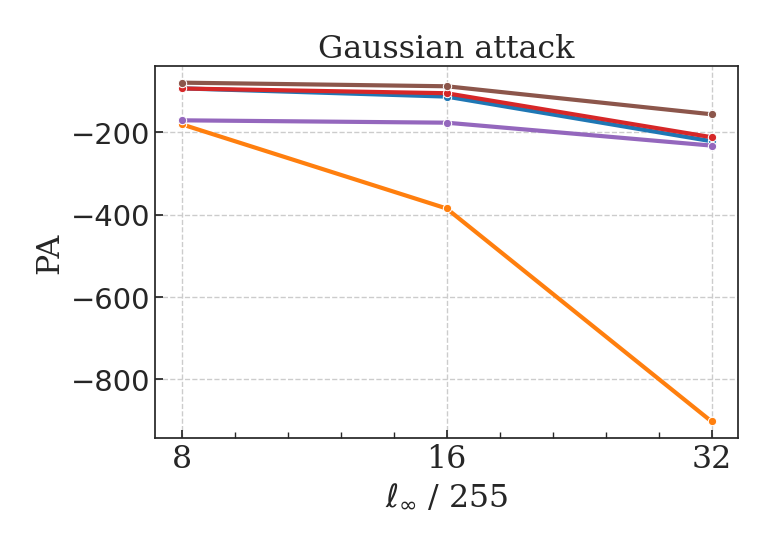
\includegraphics[width=\textwidth]{img/results_discussion/adversarial/GAUSSIAN_logPA_eps.png}
    \end{subfigure}
    \hfill
    \begin{subfigure}[b]{0.3\textwidth}
        \centering
        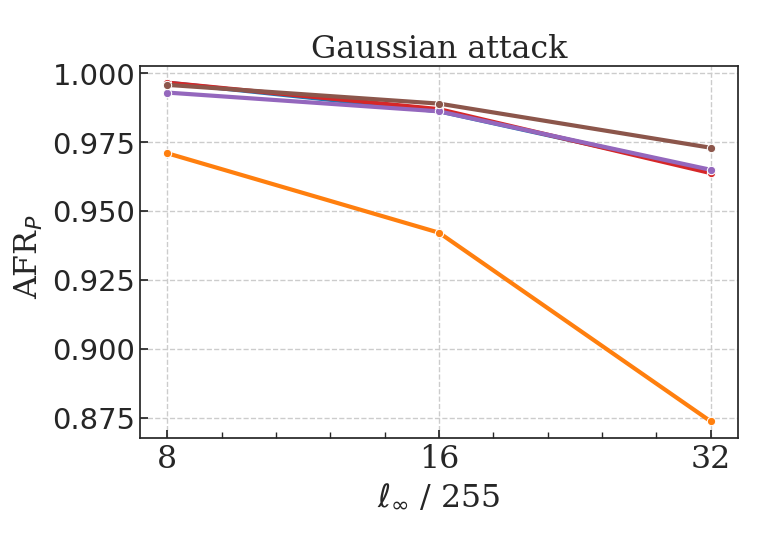
\includegraphics[width=\textwidth]{img/results_discussion/adversarial/GAUSSIAN_AFR_pred_eps.png}
    \end{subfigure}
    \hfill
    \begin{subfigure}[b]{0.3\textwidth}
        \centering
        \vspace{-5pt}
        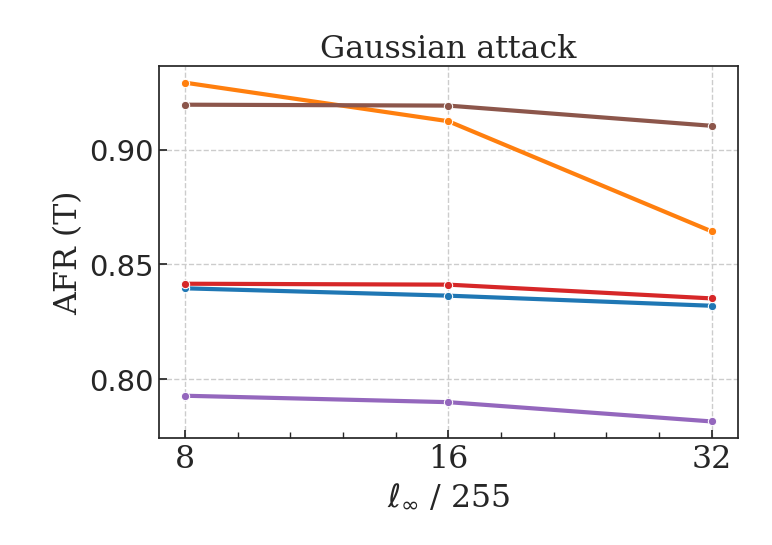
\includegraphics[width=\textwidth]{img/results_discussion/adversarial/GAUSSIAN_AFR_true_eps.png}
    \end{subfigure}
    \caption{Evolution for eps.}
    \label{fig:gaussian_optimization}
\end{figure}

MISSING: MORE DIFFERENCE BETWEEN FMN AND PGD AT FUND. LEVEL.

\section{Domain generalization setting}\label{results_domain_generalization}


\begin{figure}[H]
    \centering
    \begin{subfigure}[b]{0.3\textwidth}
        \centering
        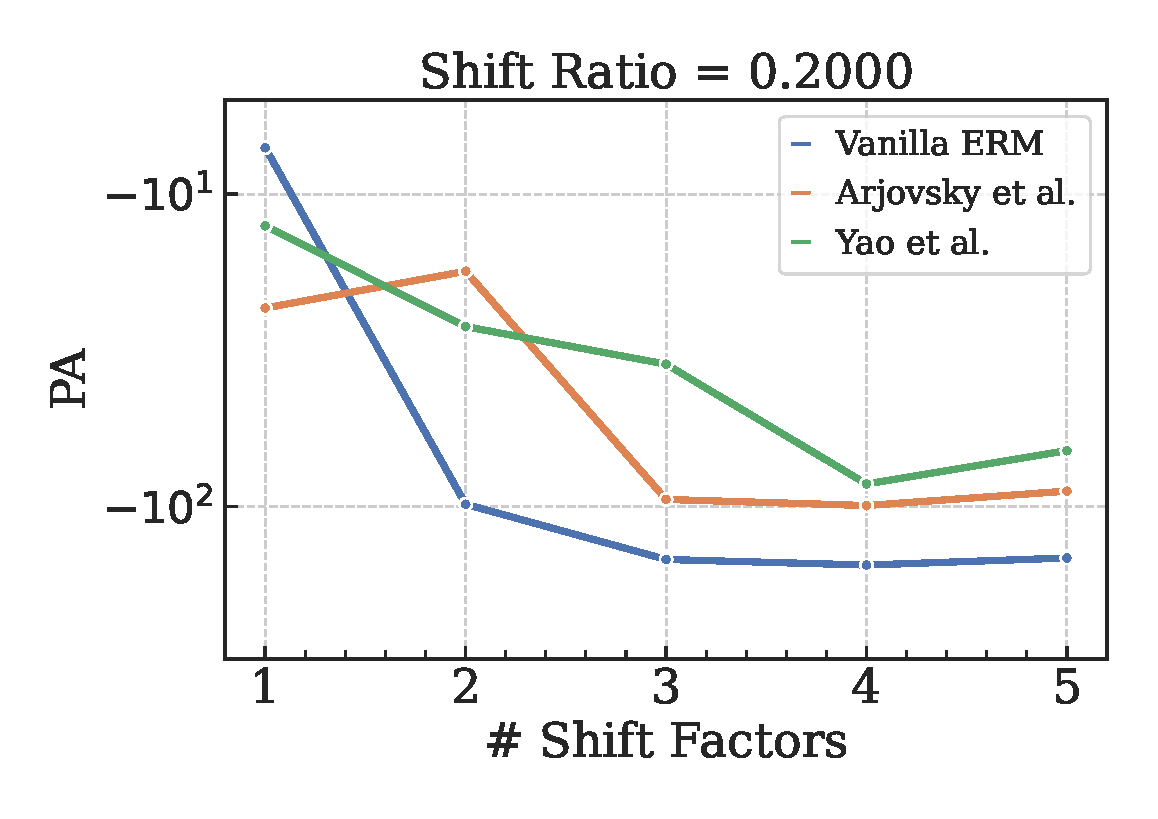
\includegraphics[width=\textwidth]{img/results_discussion/datashift/shift_ratio=0.200.pdf}
    \end{subfigure}
    \hfill
    \begin{subfigure}[b]{0.3\textwidth}
        \centering
        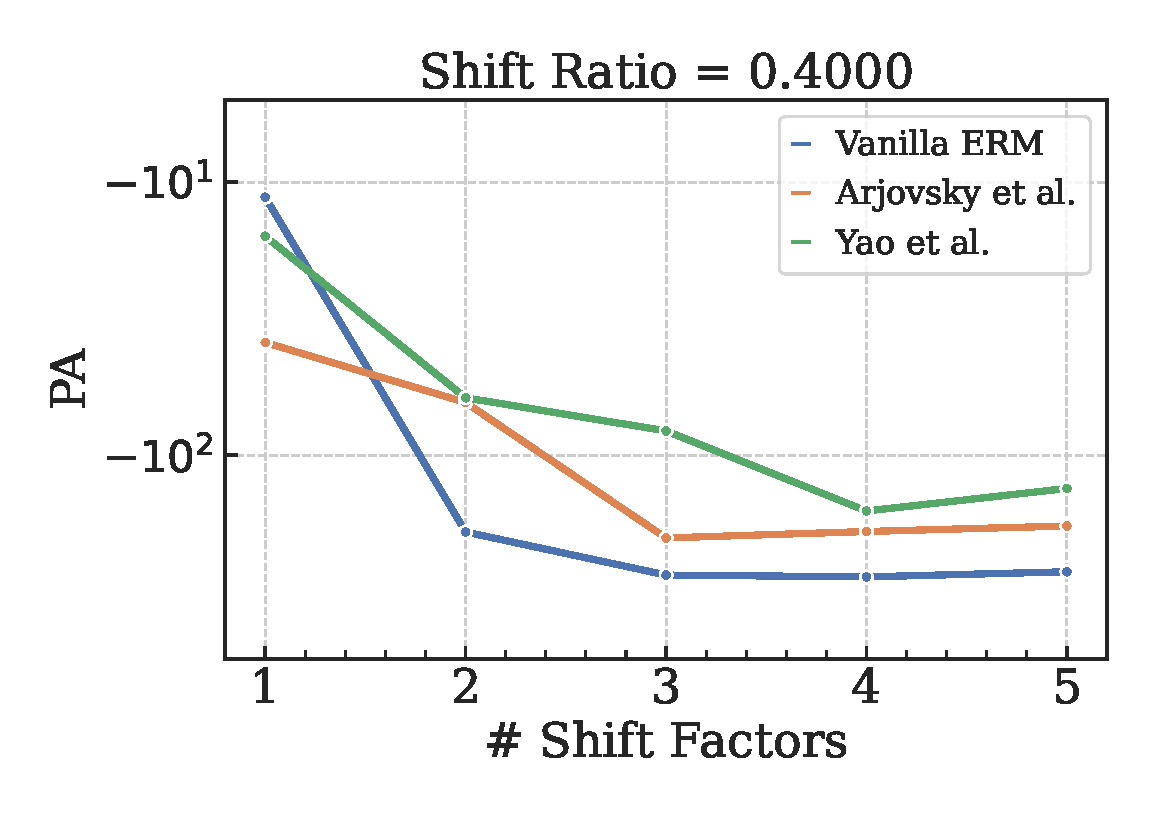
\includegraphics[width=\textwidth]{img/results_discussion/datashift/shift_ratio=0.400.pdf}
    \end{subfigure}
    \hfill
    \begin{subfigure}[b]{0.3\textwidth}
        \centering
        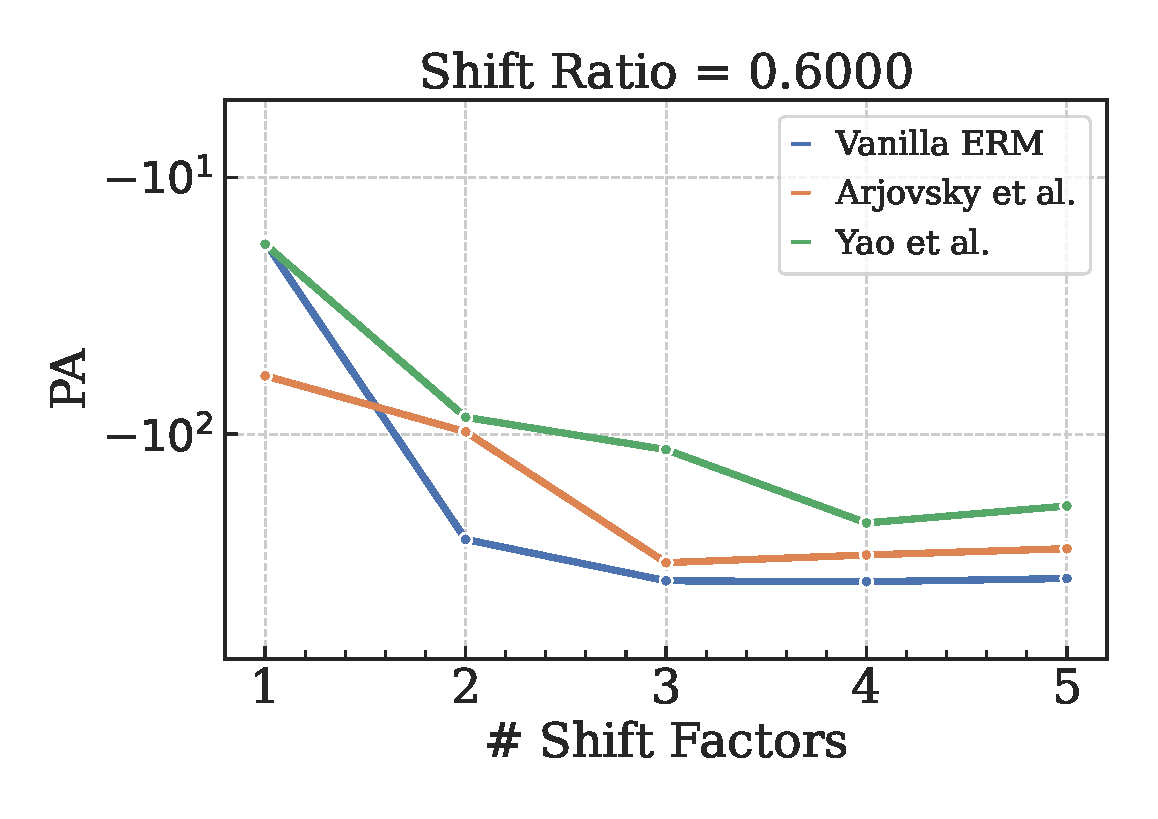
\includegraphics[width=\textwidth]{img/results_discussion/datashift/shift_ratio=0.600.pdf}
    \end{subfigure}

    \vspace{1em}

    \begin{subfigure}[b]{0.3\textwidth}
        \centering
        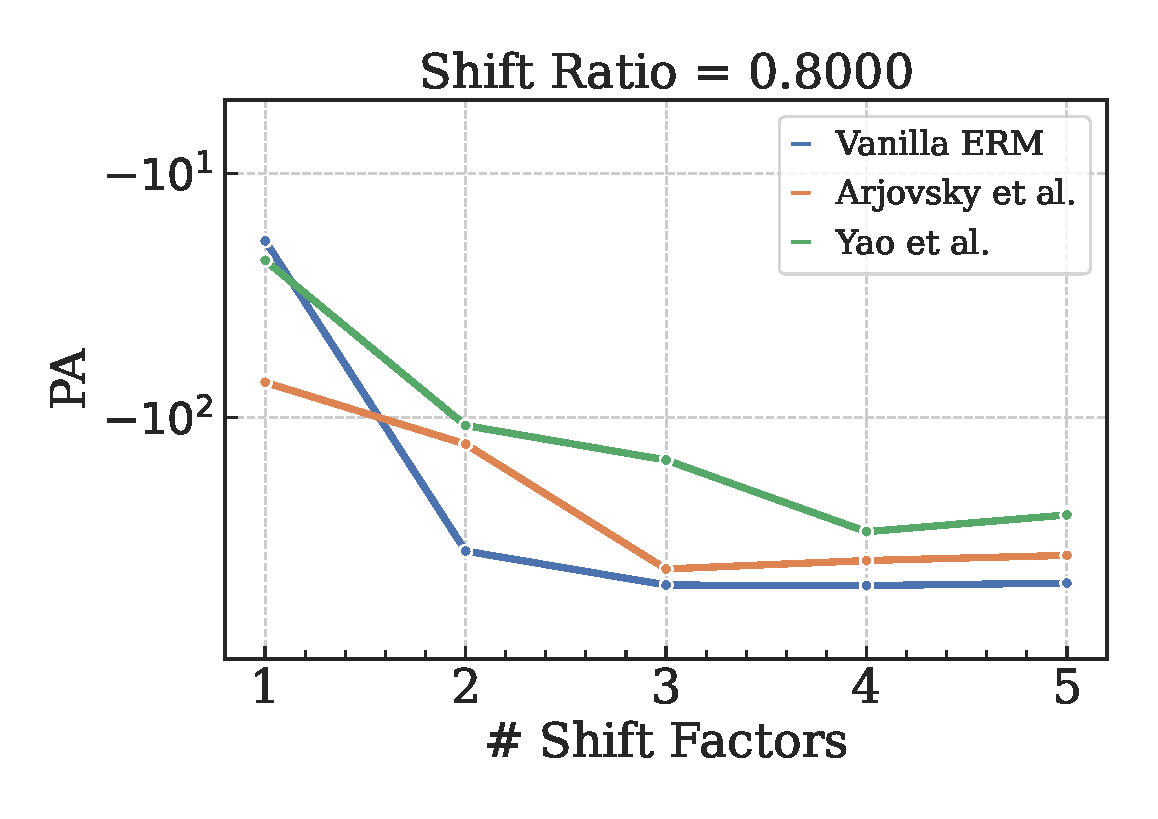
\includegraphics[width=\textwidth]{img/results_discussion/datashift/shift_ratio=0.800.pdf}
    \end{subfigure}
    \hspace{13pt}
    \begin{subfigure}[b]{0.3\textwidth}
        \centering
        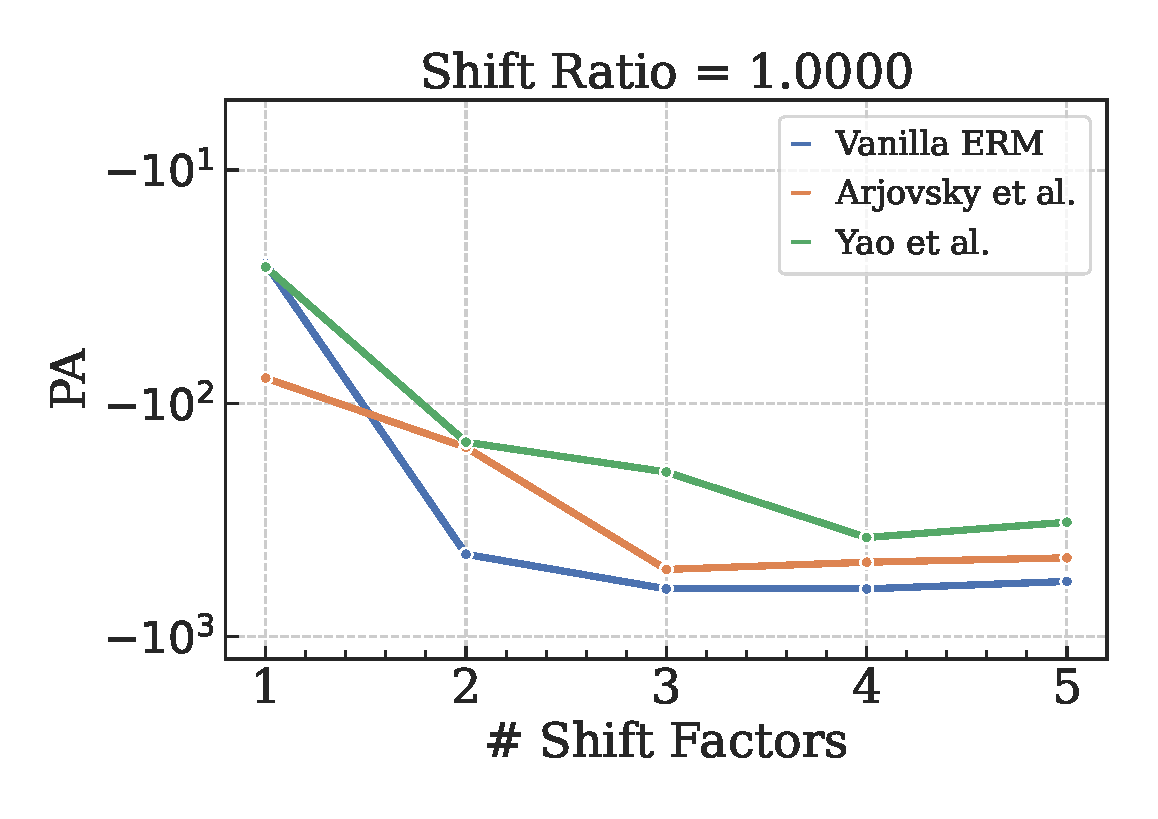
\includegraphics[width=\textwidth]{img/results_discussion/datashift/shift_ratio=1.000.pdf}
    \end{subfigure}

    \caption{Datashift for paper.}
    \label{fig:six_figures}
\end{figure}

- Adam was used to avoid a continuous pathway in the optimization landscape and therefore favouring the exploration of different solutions that might generalize better to increasingly shifted datasets.
- PA is a lower bound for accuracy, in the sense tha t

\begin{figure}[H]
    \centering
    \begin{subfigure}[b]{0.45\textwidth}
        \centering
        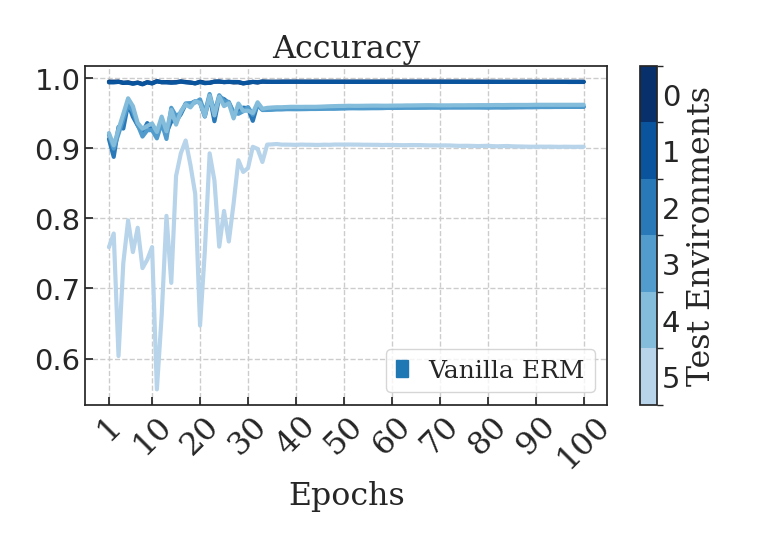
\includegraphics[width=\textwidth]{img/results_discussion/datashift/paper_oracle_all_erm.png}
    \end{subfigure}
    \hfill
    \begin{subfigure}[b]{0.45\textwidth}
        \centering
        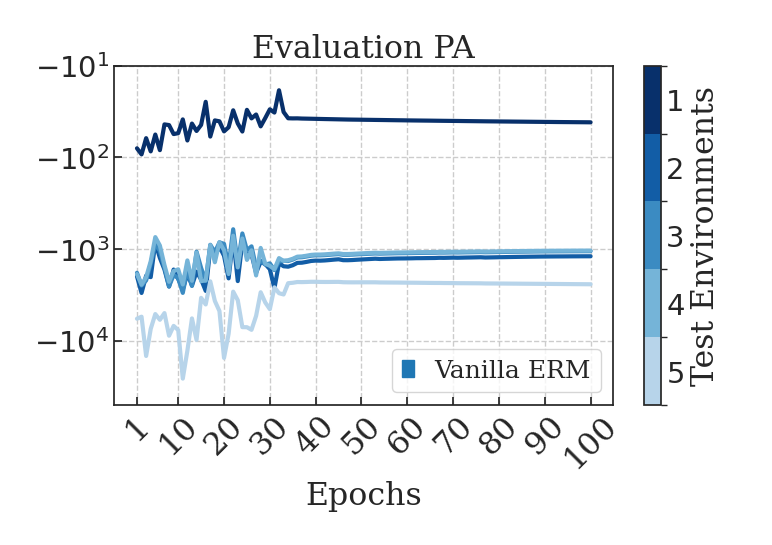
\includegraphics[width=\textwidth]{img/results_discussion/datashift/paper_PA_all_erm.png}
    \end{subfigure}

    \vspace{1em}

    \begin{subfigure}[b]{0.45\textwidth}
        \centering
        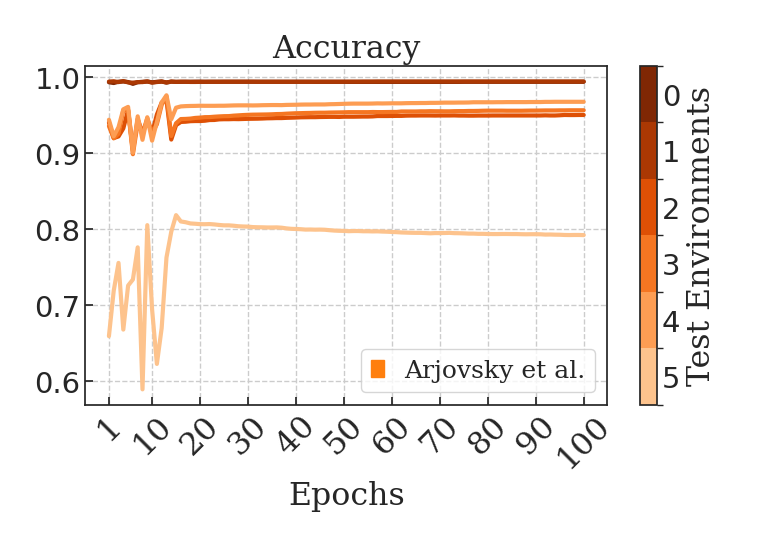
\includegraphics[width=\textwidth]{img/results_discussion/datashift/paper_oracle_all_irm.png}
    \end{subfigure}
    \hfill
    \begin{subfigure}[b]{0.45\textwidth}
        \centering
        \includegraphics[width=\textwidth]{img/results_discussion/datashift/paper_PA_all_irm.png}
    \end{subfigure}

    \caption{PA evaluation.}
    \label{fig:six_figures}
\end{figure}

\begin{figure}
    \centering
    \includegraphics[width=0.7\textwidth]{img/results_discussion/datashift/model_selection.png}
    \caption{Model selection capabilities.}
    \label{fig:model_selection_capabilities}
\end{figure}

\begin{figure}[H]
    \centering
    \begin{subfigure}[b]{0.32\textwidth}
        \centering
        \includegraphics[width=\textwidth]{img/results_discussion/datashift/paper_selection_ppred=1.0_met=acc.png}
    \end{subfigure}
    \hfill
    \begin{subfigure}[b]{0.32\textwidth}
        \centering
        \includegraphics[width=\textwidth]{img/results_discussion/datashift/paper_selection_ppred=1.0_met=sensitivity.png}
    \end{subfigure}
    \hfill
    \begin{subfigure}[b]{0.32\textwidth}
        \centering
        \vspace{-5pt}
        \includegraphics[width=\textwidth]{img/results_discussion/datashift/paper_selection_ppred=1.0_met=specificity.png}
    \end{subfigure}
    \caption{Model selection for \texttt{paper}.}
    \label{fig:gaussian_optimization}
\end{figure}



\cleardoublepage


\chapter{Discussion}\label{sec:again_something}

Blah, blah \dots

 \cleardoublepage
